\documentclass[12pt,a4paper]{article}
\usepackage[utf8]{inputenc}
\usepackage[T1]{fontenc}
\usepackage[brazil]{babel}
\usepackage{amsmath,amssymb,amsfonts}
\usepackage{graphicx}
\usepackage{geometry}
\usepackage{booktabs}
\usepackage{microtype}
\usepackage{float}
\usepackage{xcolor}
\usepackage{listings}
\usepackage{hyperref}
\usepackage{cite}

\geometry{
    a4paper,
    left=3cm,
    right=2cm,
    top=3cm,
    bottom=2cm
}

\linespread{1.25}

\hypersetup{
    colorlinks=true,
    linkcolor=black,
    citecolor=blue,
    urlcolor=blue
}

\begin{document}

\begin{titlepage}
    \centering
    \vspace*{1cm}
    {\Large \textbf{UNIVERSIDADE CATÓLICA DE SANTOS}}\\[0.3cm]
    {\large CIÊNCIA DA COMPUTAÇÃO}\\[0.3cm]
    {\large COMPUTAÇÃO GRÁFICA E PROCESSAMENTO DE IMAGENS}\\[3.5cm]
    
    {\Huge \textbf{Revisão Bibliográfica:}}\\[0.4cm]
    {\LARGE \textbf{Bloom e Efeitos de Pós-Processamento em Tempo Real}}\\[3cm]
    
    \begin{flushleft}
        \textbf{Integrantes do Grupo:}\\
        Arthur Iwankiu Castro (RA: 2822116)\\
        Enzo da Silva Passos (RA: 7047045)\\
        Francklin Roberto dos Santos Junior (RA: 9125435)\\
        Kayque de Jesus Levy Rodrigues (RA: 6593272)\\
        Miguel Nepomuceno Gil (RA: 5196718)\\
        Vitor Oliveira Christovam (RA: 2362780)\\
    \end{flushleft}
    
    \vfill
    {\large Santos -- SP}\\
    {\large 2026}
\end{titlepage}

\section*{Resumo}
Este trabalho apresenta uma pesquisa teórica e bibliográfica sobre a fundamentação física, a modelagem matemática e a implementação prática do efeito de \textit{Bloom} e dos pipelines de pós-processamento em computação gráfica em tempo real. Discutem-se os princípios ópticos e fisiológicos da dispersão luminosa intraocular e em lentes fotográficas, a extração analítica de luminância com transição contínua (\textit{soft knee}), a decomposição de convoluções Gaussianas e piramidais, bem como a compressão por mapeamento tonal (\textit{tone mapping}). Detalha-se a arquitetura de implementação sob a API de baixo nível Vulkan, cobrindo o uso de \textit{Fullscreen Triangles}, transições de layout de imagem e barreiras de memória explícitas. Por fim, analisam-se aplicações em motores gráficos e realizam-se estudos de caso analíticos com capturas de tela obtidas durante o gameplay em \textit{Portal with RTX} e \textit{Cyberpunk 2077}. Na segunda etapa do trabalho, apresenta-se o desenho técnico da arquitetura do pipeline Vulkan da técnica, com seus \textit{render passes}, \textit{descriptor sets}, \textit{buffers}, \textit{shaders}, barreiras de memória e transições de \textit{layout} de imagem. Na terceira etapa, apresenta-se o pseudocódigo, em sintaxe GLSL, dos \textit{shaders} desse pipeline, com a explicação de suas entradas, saídas, cálculos, \textit{loops}, condições e amostragens de textura. Na quarta etapa, apresenta-se a implementação do \textit{boilerplate} funcional em C++ sob a API Vulkan, cobrindo o gerenciamento modular de janelas, dispositivos lógicos, \textit{swapchain}, pipeline gráfico, sincronização e a integração prática dos \textit{shaders} compilados em SPIR-V com comprovação de renderização visual. Por fim, na quinta etapa, apresenta-se o protótipo funcional completo em tempo real, integrando a cena tridimensional HDR, extração analítica de luminância, pirâmide de reduções e ampliações com mistura aditiva, composição com mapeamento tonal de Reinhard e controles interativos de teclado com validação comparativa.

\vspace{1cm}

\section{Introdução}
A renderização e exibição fidedigna de fenômenos luminosos em computação gráfica em tempo real enfrenta uma severa limitação de natureza física e tecnológica: a faixa dinâmica restrita (\textit{Low Dynamic Range} -- LDR) dos monitores de exibição convencionais \cite{seetzen2004hdr}. Enquanto tais dispositivos operam normalizados no intervalo $[0, 1]$, fontes luminosas no mundo físico (como arcos elétricos, filamentos incandescentes e o Sol) emitem radiação com ordens de magnitude substancialmente superiores às de superfícies puramente difusas circundantes \cite{seetzen2004hdr}.

Para mitigar a perda de contraste perceptivo sem saturar indiscriminadamente todo o sinal cromático da cena, a computação gráfica moderna emprega filtros espaciais em espaço de tela (\textit{screen-space}) através de passes de pós-processamento \cite{cadik2005naturalness}. Dentre esses, o \textit{Bloom} desempenha um papel essencial ao simular computacionalmente os efeitos ópticos de difração e dispersão que ocorrem naturalmente no humor vítreo e no cristalino do olho humano ou nos elementos de lentes de câmeras fotográficas \cite{spencer1995glare, cadik2005naturalness}.

\section{Explicação Teórica da Técnica}

\subsection{Definição e Objetivo}
O \textit{Bloom} (frequentemente tratado na literatura como \textit{glare} ou \textit{light bleeding}) consiste na simulação computacional do espalhamento difuso de fótons quando estes atravessam meios ópticos imperfeitos \cite{spencer1995glare}. Seu objetivo primordial é transmitir ao observador a percepção de intensidade extrema em fontes emissivas ou reflexões especulares, sobrepujando a incapacidade física dos displays de emitir luminância superior ao seu limiar nativo de brilho \cite{cadik2005naturalness}.

\subsection{Como a Técnica Funciona}
\label{sec:funciona}
O pipeline clássico de pós-processamento para geração do \textit{Bloom} opera em quatro fases ordenadas:
\begin{enumerate}
    \item \textbf{Bright Pass (Isolamento de Altas Luzes):} Realiza uma varredura sobre o \textit{framebuffer} HDR da cena, isolando e filtrando os fragmentos cuja intensidade de luminância ultrapassa um determinado limiar de corte (\textit{threshold}).
    \item \textbf{Downsampling e Filtragem Espacial:} Redução piramidal progressiva da resolução da textura isolada combinada à aplicação encadeada de filtros de desfoque espacial (como convoluções Gaussianas ou pirâmides de filtragem), gerando múltiplos níveis de dispersão com raios variados \cite{cadik2005naturalness}.
    \item \textbf{Upsampling e Composição Aditiva:} Interpolação bilinear progressiva das camadas desfocadas da menor para a maior resolução, acumulando aditivamente as contribuições espalhadas sobre a imagem original da cena.
    \item \textbf{Tone Mapping (Mapeamento Tonal):} Compressão matemática da imagem HDR combinada para o intervalo $[0, 1]$ aceito pelos dispositivos LDR, preservando detalhes tanto em penumbra quanto em altas claridades \cite{reinhard2002tone}.
\end{enumerate}

\subsection{Problema Resolvido, Vantagens e Limitações}
A técnica soluciona a perda de contraste perceptivo em que superfícies brancas puras $(1.0, 1.0, 1.0)$ e fontes ativamente incandescentes seriam representadas com idêntico valor após a rasterização direta.

\textbf{Vantagens:} Apresenta custo computacional reduzido e previsível, operando estritamente em espaço de tela 2D após a resolução da geometria tridimensional.

\textbf{Limitações:} A calibração inadequada de limiar ou do raio de espalhamento pode introduzir embaçamento generalizado (\textit{haze}), saturação excessiva e perda de nitidez estrutural dos modelos 3D.

\subsection{Custo Computacional e Aplicação Adequada}
\label{sec:custo}
O processamento independe da complexidade geométrica, contagem de polígonos ou complexidade de materiais da cena, apresentando custo temporal puramente linear $\mathcal{O}(P)$, onde $P$ é o total de pixels processados. É indispensável para cenas noturnas com iluminação artificial, cenas externas sob luz solar direta e jogos com superfícies altamente reflexivas.

\section{Equações Matemáticas Envolvidas}
\label{sec:equacoes}

\subsection{Luminância Perceptual (Espaço ITU-R BT.709)}
A filtragem de fragmentos candentes fundamenta-se na sensibilidade espectral da visão humana, que prioriza a faixa espectral do verde:
\begin{equation}
    L = 0.2126\,R + 0.7152\,G + 0.0722\,B
    \label{eq:luminancia}
\end{equation}
\textbf{Significado das variáveis:}
\begin{itemize}
    \item $R, G, B$: Canais lineares de cor com precisão de ponto flutuante (\textit{floating-point}).
    \item $L$: Luminância escalar perceptual calculada para o fragmento.
\end{itemize}
\textbf{Momento de uso e relação com a renderização:} Utilizada na etapa preliminar de \textit{Bright Pass} para avaliar quais fragmentos possuem energia suficiente para gerar halos de dispersão.

\subsection{Extração com Joelho Suave (\textit{Bright-Pass Soft Knee})}
Para evitar descontinuidades e ruídos de cintilação temporal (\textit{fireflies}) ao longo de bordas móveis, emprega-se uma função de transição contínua com joelho suave:
\begin{equation}
    C_{\text{bright}} = C_{\text{cena}} \cdot \frac{\max\left(0, \min(L - T + k, 2k)\right)^2}{4k + \epsilon}
    \label{eq:softknee}
\end{equation}
\textbf{Significado das variáveis:}
\begin{itemize}
    \item $C_{\text{cena}}$: Vetor tridimensional de cor HDR original do pixel.
    \item $T$: Limiar de corte (\textit{threshold}) estipulado artisticamente.
    \item $k$: Fator escalar de abertura da transição suave (\textit{knee}).
    \item $\epsilon$: Constante infinitesimal para evitar divisões por zero.
    \item $C_{\text{bright}}$: Vetor de cor filtrado que alimenta as etapas subsequentes de convolução.
\end{itemize}
\textbf{Momento de uso e relação com a renderização:} Executada no \textit{Fragment Shader} ou \textit{Compute Shader} que gera o primeiro nível de resolução da cadeia de dispersão.

\subsection{Função de Espalhamento Pontual de Spencer (\textit{Point Spread Function})}
A base biofísica da dispersão de luz decorrente de micropartículas no olho humano foi formalizada por Spencer et al. \cite{spencer1995glare}:
\begin{equation}
    f(\theta) = \frac{k_1}{\theta^3 + \epsilon} + \frac{k_2}{\theta^2}
    \label{eq:psf}
\end{equation}
\textbf{Significado das variáveis:}
\begin{itemize}
    \item $\theta$: Ângulo de desvio angular da linha direta de visada em radianos.
    \item $k_1, k_2$: Coeficientes empíricos relacionados à difração no cristalino e à dispersão na córnea.
    \item $\epsilon$: Termo de amortecimento que evita singularidades numéricas quando $\theta \to 0$.
\end{itemize}
\textbf{Momento de uso e relação com a renderização:} Constitui o embasamento físico do fenômeno; por ter cálculo integral contínuo custoso, é discretizada mediante múltiplos passos de filtragem espacial \cite{cadik2005naturalness}.

\subsection{Kernel Gaussiano Separável Unidimensional}
A discretização em tempo real da PSF efetua-se decompondo o filtro bidimensional em dois passos ortogonais (horizontal e vertical), barateando o custo por pixel de $\mathcal{O}(K^2)$ para $\mathcal{O}(2K)$:
\begin{equation}
    G(x) = \frac{1}{\sqrt{2\pi\sigma^2}} \exp\left(-\frac{x^2}{2\sigma^2}\right)
    \label{eq:gauss}
\end{equation}
\textbf{Significado das variáveis:}
\begin{itemize}
    \item $x$: Deslocamento discreto em coordenadas de \textit{texels} a partir do centro da convolução.
    \item $\sigma$: Desvio padrão da distribuição Gaussiana, definidor do raio de dispersão luminosa.
\end{itemize}
\textbf{Momento de uso e relação com a renderização:} Aplicada a cada nível da cadeia de amostragem regressiva (\textit{downsampling}) e progressiva (\textit{upsampling}) para expandir o halo de brilho.

\subsection{Mapeamento Tonal Fotográfico de Reinhard}
Para recombinar o brilho acumulado à imagem da cena e comprimir a faixa dinâmica sem achatamento abrupto, emprega-se a formulação de Reinhard et al. \cite{reinhard2002tone}:
\begin{equation}
    C_{\text{final}} = \frac{C_{\text{total}}}{1 + C_{\text{total}}}, \quad \text{onde } C_{\text{total}} = C_{\text{cena}} + \alpha C_{\text{bloom}}
    \label{eq:reinhard}
\end{equation}
\textbf{Significado das variáveis:}
\begin{itemize}
    \item $C_{\text{cena}}$: Cor HDR original da cena renderizada.
    \item $C_{\text{bloom}}$: Contribuição de cor acumulada pela pirâmide de dispersão.
    \item $\alpha$: Parâmetro multiplicativo de calibração da intensidade do \textit{Bloom}.
    \item $C_{\text{final}}$: Sinal cromático mapeado para o intervalo normalizado $[0, 1]$.
\end{itemize}
\textbf{Momento de uso e relação com a renderização:} Etapa final do pipeline de pós-processamento, antecedendo o envio do \textit{framebuffer} ao \textit{Swapchain}.

\section{Relação da Técnica com a API Vulkan}
\label{sec:vulkan}

\subsection{Shaders e Pipelines Gráficos}
A arquitetura do \textit{Bloom} no Vulkan implementa-se de forma enxuta sem necessidade de alocação de malhas ou \textit{Vertex Buffers}:
\begin{itemize}
    \item \textbf{Fullscreen Triangle:} O \textit{Vertex Shader} gera um triângulo analítico único diretamente a partir do identificador intrínseco \texttt{gl\_VertexIndex}. O polígono recobre integralmente o espaço de coordenadas de tela (NDC), suprimindo os custos de interpolação duplicada na diagonal característicos de quads tradicionais.
    \item \textbf{Compute Shaders e Memória Compartilhada:} Nos passos de convolução, agrupam-se \textit{threads} em grupos locais (\textit{workgroups} de $16 \times 16$). Os dados dos \textit{texels} vizinhos são carregados em memória compartilhada (\textit{shared memory} / LDS), contornando leituras redundantes na VRAM e maximizando a vazão de registradores da GPU.
\end{itemize}

\subsection{Buffers, Attachments e Sincronização}
O fluxo de dados transita sequencialmente:\\
\texttt{Cena HDR} $\to$ \texttt{Bright Pass} $\to$ \texttt{Mip Chain (Down)} $\to$ \texttt{Upsample (Tent Filter)} $\to$ \texttt{Tone Mapping} $\to$ \texttt{Swapchain}.

O \textit{framebuffer} primário requer formatos em ponto flutuante de 16 ou 32 bits, comumente:
\begin{center}
    \texttt{VK\_FORMAT\_R16G16B16A16\_SFLOAT}
\end{center}
As texturas alocadas para a pirâmide de resolução demandam o uso simultâneo de sinalizadores na estrutura \texttt{VkImageCreateInfo}:
\begin{center}
    \texttt{VK\_IMAGE\_USAGE\_COLOR\_ATTACHMENT\_BIT | VK\_IMAGE\_USAGE\_SAMPLED\_BIT | VK\_IMAGE\_USAGE\_STORAGE\_BIT}
\end{center}
\begin{sloppypar}
\noindent A alternância segura entre etapas de escrita e leitura nos múltiplos níveis é coordenada por barreiras de sincronização explícitas (\texttt{vkCmdPipelineBarrier}), que efetuam transições de \texttt{VK\_\allowbreak IMAGE\_\allowbreak LAYOUT\_\allowbreak COLOR\_\allowbreak ATTACHMENT\_\allowbreak OPTIMAL} para \texttt{VK\_\allowbreak IMAGE\_\allowbreak LAYOUT\_\allowbreak SHADER\_\allowbreak READ\_\allowbreak ONLY\_\allowbreak OPTIMAL}, estabelecendo dependências estritas entre os estágios \texttt{VK\_\allowbreak PIPELINE\_\allowbreak STAGE\_\allowbreak COLOR\_\allowbreak ATTACHMENT\_\allowbreak OUTPUT\_\allowbreak BIT} e \texttt{VK\_\allowbreak PIPELINE\_\allowbreak STAGE\_\allowbreak FRAGMENT\_\allowbreak SHADER\_\allowbreak BIT}.
\end{sloppypar}

\section{Aplicações Práticas}
\begin{itemize}
    \item \textbf{NVIDIA RTX Remix:} No pipeline modular de traçado de caminhos em tempo real (\textit{Path Tracing}), o \textit{Bloom} atua subsequentemente ao desruído temporal, atenuando transições de alto contraste e dispersando a energia de emissores de radiação física sobre superfícies vizinhas em espaço de tela \cite{ignatenko2008glare}.
    \item \textbf{Unreal Engine 5:} Integração de desfoque convolucional de abertura física com o sistema de iluminação global dinâmica Lumen, conferindo volume perceptivo e legibilidade visual a materiais emissivos em ambientes de penumbra.
\end{itemize}

\section{Análise da Técnica em Jogos}

\subsection{Jogo 1: Portal with RTX}
\begin{itemize}
    \item \textbf{Nome do jogo e Plataforma:} \textit{Portal with RTX}, executado em computador pessoal com sistema operacional Windows 11.
    \item \textbf{Situação de gameplay analisada:} Câmara de testes durante o disparo e trânsito da esfera de energia de alta densidade (\textit{High Energy Pellet}) próxima às paredes metálicas modulares reflexivas.
    \item \textbf{Momento em que a técnica pode ser observada:} No instante em que o projétil incandescente cruza a sala e se aproxima da superfície metálica vertical da câmara de testes.
    \item \textbf{Elemento visual de aplicação:} Esfera emissora de plasma em movimento no ar e a superfície modular metálica da parede adjacente.
    \item \textbf{Efeito visual produzido:} O projétil pontual de plasma (círculo ciano) gera um halo volumétrico difuso e intenso que ultrapassa a geometria do objeto em direção à visão do jogador; simultaneamente, o reflexo especular refletido nas placas facetadas da parede (círculo vermelho) acumula luminância suficiente para ativar o filtro de \textit{Bright Pass}, transbordando um gradiente de sangramento de luz (\textit{light bleeding}) sobre as costuras escuras dos painéis vizinhos.
    \item \textbf{Benefício da técnica para o jogo:} Transmite a sensação tátil de perigo e calor concentrado da esfera de plasma, evitando que o reflexo especular pareça uma mancha opaca e integrando a iluminação por traçado de caminhos (\textit{Path Tracing}) aos limites de contraste do monitor.
    \item \textbf{Fonte técnica confirmatória:} A formulação de filtros em espaço de tela (\textit{image-space}), isolamento de altas intensidades e aceleração de dispersão luminosa em pipelines HDR descrita por Ignatenko e Barladyan \cite{ignatenko2008glare}.
\end{itemize}

\begin{figure}[H]
    \centering
    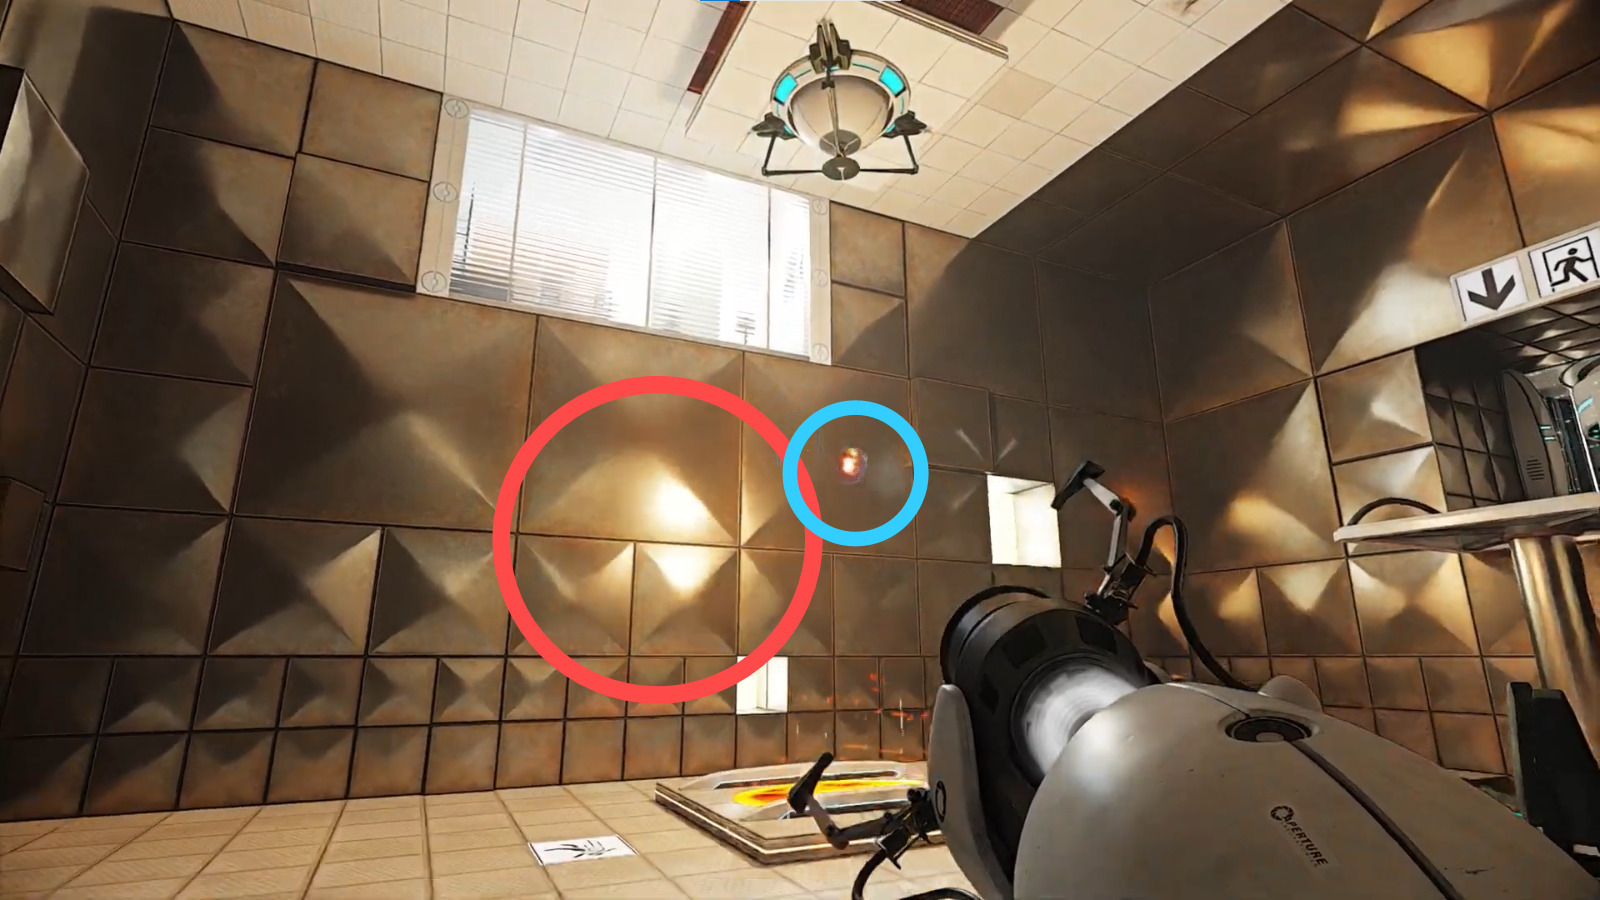
\includegraphics[width=0.88\textwidth]{figura1.jpg}
    \caption{Captura de tela obtida durante o gameplay de \textit{Portal with RTX}. O círculo ciano destaca o projétil de plasma incandescente em trânsito com saturação no núcleo e halo de dispersão; o círculo vermelho evidencia o reflexo especular de alta intensidade na parede metálica com sangramento de luz (\textit{light bleeding}) sobre as junções dos painéis.}
    \label{fig:portal}
\end{figure}
\subsection{Jogo 2: Cyberpunk 2077}
\begin{itemize}
    \item \textbf{Nome do jogo e Plataforma:} \textit{Cyberpunk 2077}, executado em computador pessoal (PC/Windows 11) sobre o motor gráfico REDengine 4.
    \item \textbf{Situação de gameplay analisada:} Exploração noturna a pé no distrito urbano em frente ao estabelecimento comercial \textit{Lizzie's Bar}, em ambiente com alta concentração de fontes emissivas de néon e piso asfáltico molhado com reflexões especulares.
    \item \textbf{Momento em que a técnica pode ser observada:} No momento em que a visão do jogador mira a fachada iluminada com luminosos de néon e as poças de chuva refletoras na via pública.
    \item \textbf{Elemento visual de aplicação:} Painel publicitário emissivo superior (\textit{WET DREAM}), silhuetas figurativas de néon na fachada e reflexos diretos no chão molhado.
    \item \textbf{Efeito visual produzido:} O painel publicitário de alta luminância (demarcado pelo círculo ciano) gera um halo de dispersão volumétrica que transborda os limites da tela. Simultaneamente, as silhuetas de néon (círculo magenta) e as reflexões no piso (círculo vermelho) produzem sangramento cromático suave sobre a dispersão atmosférica ambiente (retângulo amarelo).
    \item \textbf{Benefício da técnica para o jogo:} Essencial para conferir a atmosfera densa e visualmente distópica do cenário urbano futurista, transmitindo a intensidade física das luzes artificiais contra a noite e ampliando a percepção de contraste.
    \item \textbf{Fonte técnica confirmatória:} O modelo de avaliação perceptiva e simulação de dispersão luminosa (\textit{glare}) em imagens HDR detalhado por Čadík et al. \cite{cadik2005naturalness}.
\end{itemize}

\begin{figure}[H]
    \centering
    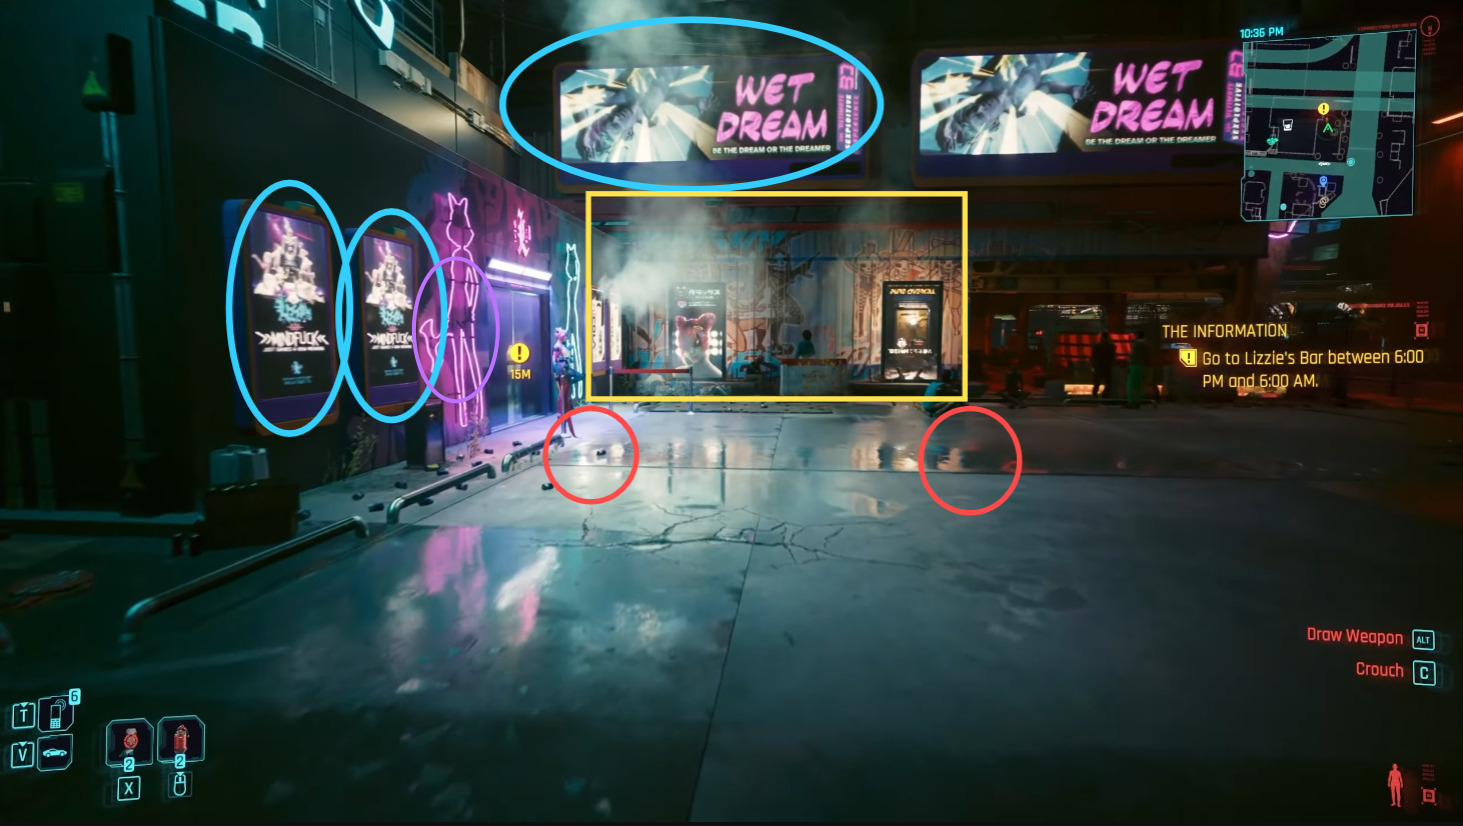
\includegraphics[width=0.88\textwidth]{figura2.jpg}
    \caption{Captura de tela obtida durante a execução do gameplay de \textit{Cyberpunk 2077}. O círculo ciano isola o painel emissivo principal (\textit{WET DREAM}); o círculo magenta demarca a iluminação de néon da fachada; o retângulo amarelo indica a dispersão difusa na névoa ambiente; o círculo vermelho destaca o sangramento de luz na reflexão especular do solo molhado.}
    \label{fig:cyberpunk}
\end{figure}

% Entrega 2: arquitetura do pipeline Vulkan
% ===============================================================
% Entrega 2: Arquitetura do Pipeline Vulkan (Bloom)
% Este arquivo e incluido no main.tex com % ===============================================================
% Entrega 2: Arquitetura do Pipeline Vulkan (Bloom)
% Este arquivo e incluido no main.tex com % ===============================================================
% Entrega 2: Arquitetura do Pipeline Vulkan (Bloom)
% Este arquivo e incluido no main.tex com \input{entrega2}
% ===============================================================

\section{Arquitetura do Pipeline Vulkan}
\label{sec:arquitetura}
\sloppy

Esta seção é a segunda entrega do trabalho. A Figura~\ref{fig:pipeline} mostra o desenho do pipeline Vulkan que executa o \textit{Bloom}, feito no draw.io. Como exemplo, o grupo considerou uma tela de $1920 \times 1080$, imagens no formato \texttt{VK\_FORMAT\_R16G16B16A16\_SFLOAT}, citado na Seção~\ref{sec:vulkan}, e uma pirâmide de cinco níveis, de \texttt{bloomMip[0]} a \texttt{bloomMip[4]}.

\begin{figure}[H]
    \centering
    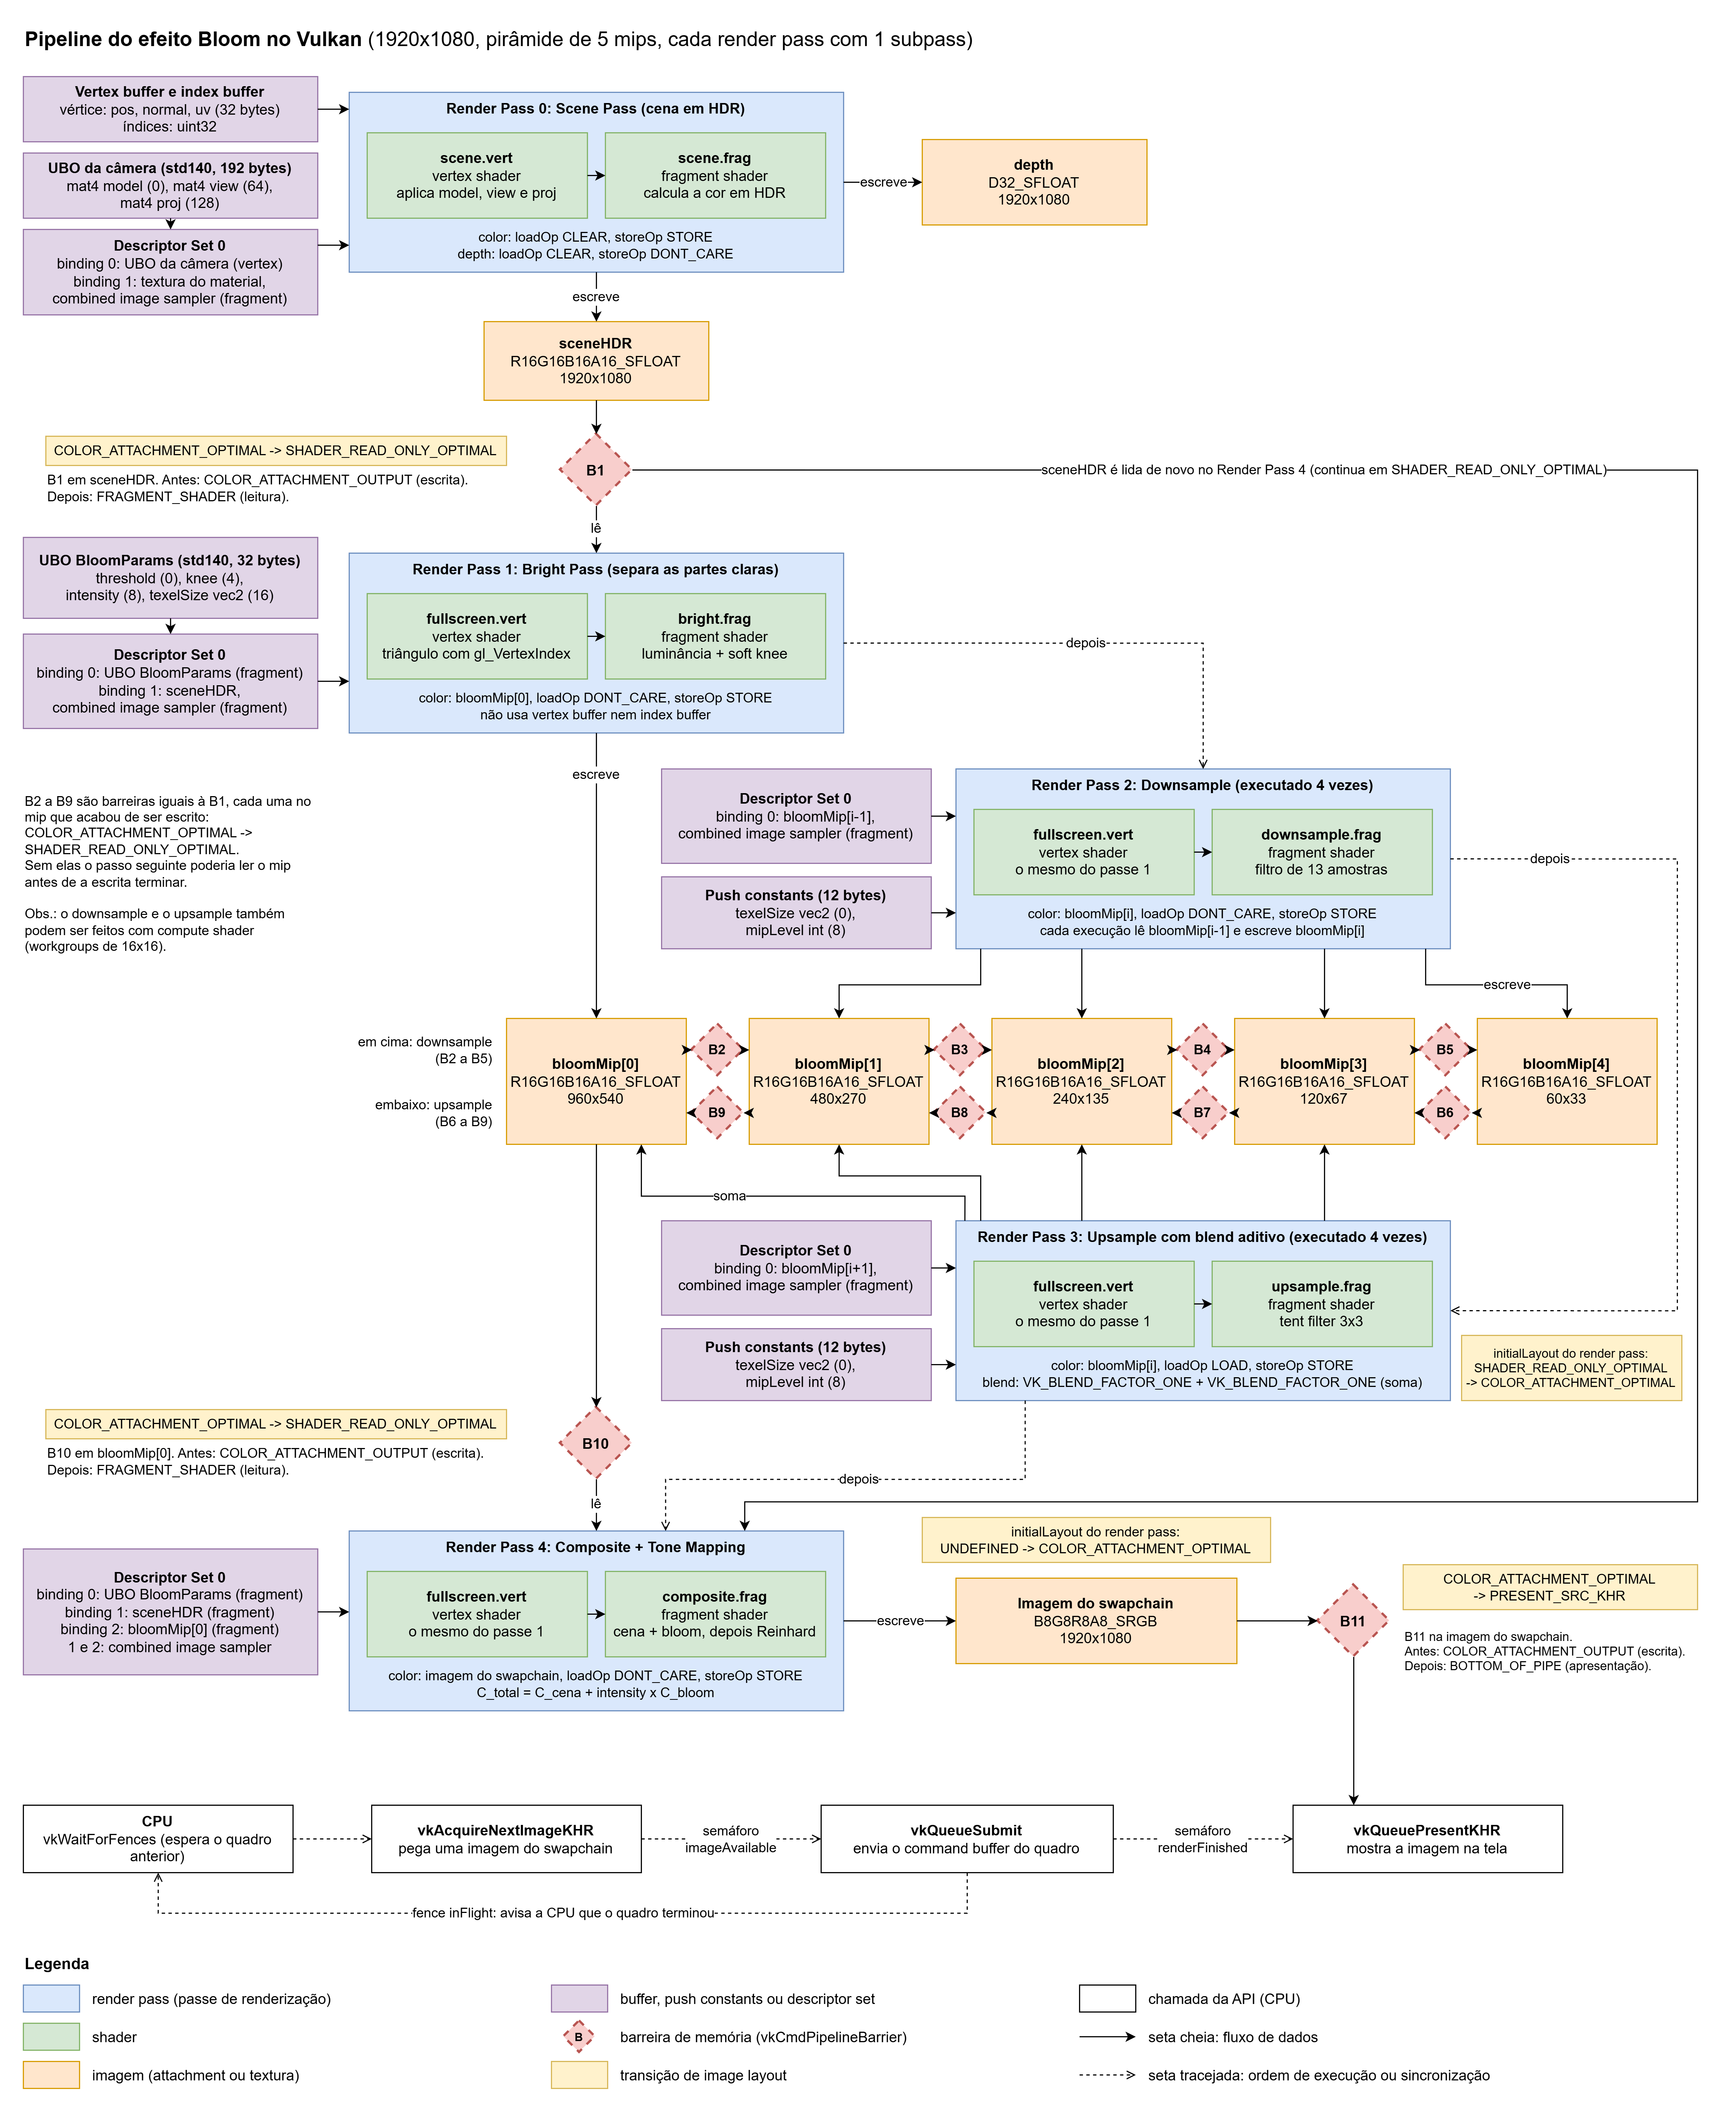
\includegraphics[height=0.64\textheight]{diagrama.png}
    \caption{Arquitetura do pipeline Vulkan para o efeito de \textit{Bloom}. Azul: \textit{render pass}. Verde: \textit{shader}. Laranja: imagem. Roxo: \textit{buffer} ou \textit{descriptor set}. Losango vermelho: barreira de memória. Amarelo: transição de \textit{layout}. Seta cheia: dados. Seta tracejada: ordem de execução ou sincronização.}
    \label{fig:pipeline}
\end{figure}

\subsection{Fluxo de Dados}
O quadro é desenhado em onze passes, gravados em ordem em um único \textit{command buffer}:
\begin{enumerate}
    \setlength{\itemsep}{0pt}
    \item \textbf{Passe 0 (\textit{Scene Pass}):} recebe o \textit{vertex buffer}, o \textit{index buffer}, o UBO da câmera e as texturas. Desenha a cena na \texttt{sceneHDR}, usando a \texttt{depth} no teste de profundidade.
    \item \textbf{Passe 1 (\textit{Bright Pass}):} lê a \texttt{sceneHDR} e guarda só as partes claras na \texttt{bloomMip[0]}, com metade da resolução.
    \item \textbf{Passes 2 a 5 (\textit{Downsample}):} cada execução lê \texttt{bloomMip[i-1]} e escreve \texttt{bloomMip[i]}, menor e mais borrado.
    \item \textbf{Passes 6 a 9 (\textit{Upsample}):} cada execução lê \texttt{bloomMip[i+1]} e soma o resultado em \texttt{bloomMip[i]}. No fim, a \texttt{bloomMip[0]} tem o halo completo.
    \item \textbf{Passe 10 (\textit{Composite}):} soma a \texttt{sceneHDR} com a \texttt{bloomMip[0]}, aplica o \textit{tone mapping} e escreve na imagem do \textit{swapchain}, que é mostrada na tela.
\end{enumerate}
\textbf{Recursos compartilhados.} A \texttt{sceneHDR} é lida nos passes 1 e 10. Os níveis \texttt{bloomMip} são \textit{mip levels} de uma mesma \texttt{VkImage}, usados na descida e na subida. O UBO \texttt{BloomParams} serve aos passes 1 e 10, e o \texttt{fullscreen.vert} e o \texttt{VkSampler} são os mesmos em todos os passes de tela cheia.

\subsection{Render Passes e Subpasses}
São cinco \textit{render passes}, todos com um único \textit{subpass} (Tabela~\ref{tab:renderpasses}).

\begin{table}[H]
    \centering
    \caption{\textit{Render passes} do pipeline.}
    \label{tab:renderpasses}
    \vspace{4pt}
    \scriptsize
    \setlength{\tabcolsep}{4pt}
    \begin{tabular}{c c l l l l}
        \toprule
        \textbf{RP} & \textbf{Passes} & \textbf{Attachment} & \textbf{loadOp / storeOp} & \textbf{initialLayout} & \textbf{Resultado} \\
        \midrule
        0 & 0 & \texttt{sceneHDR} (cor) & \texttt{CLEAR / STORE} & \texttt{UNDEFINED} & cena em HDR \\
          &   & \texttt{depth} (profundidade) & \texttt{CLEAR / DONT\_CARE} & \texttt{UNDEFINED} & teste de profundidade \\
        1 & 1 & \texttt{bloomMip[0]} & \texttt{DONT\_CARE / STORE} & \texttt{UNDEFINED} & partes claras da cena \\
        2 & 2 a 5 & \texttt{bloomMip[1]} a \texttt{bloomMip[4]} & \texttt{DONT\_CARE / STORE} & \texttt{UNDEFINED} & nível menor e borrado \\
        3 & 6 a 9 & \texttt{bloomMip[3]} a \texttt{bloomMip[0]} & \texttt{LOAD / STORE} & \texttt{SHADER\_READ\_ONLY\_OPTIMAL} & soma dos níveis \\
        4 & 10 & imagem do \textit{swapchain} & \texttt{DONT\_CARE / STORE} & \texttt{UNDEFINED} & imagem final \\
        \bottomrule
    \end{tabular}
\end{table}

No início do \textit{subpass}, o \textit{render pass} leva o \textit{attachment} do \texttt{initialLayout} para \texttt{COLOR\_ATTACHMENT\_OPTIMAL}. O \textit{upsample} usa \texttt{LOAD} porque precisa manter o conteúdo anterior para a soma. Os passes ficaram em \textit{render passes} separados porque cada um escreve em uma imagem de tamanho diferente e lê \textit{texels} vizinhos da anterior com um \textit{sampler}, o que um \textit{input attachment} não permite. O \texttt{VK\_KHR\_dynamic\_rendering} não foi usado por não ser o modelo visto na disciplina.

\subsection{Descriptor Sets e Bindings}
Todos os pipelines usam só o \textit{set} 0 (Tabela~\ref{tab:descriptors}). No \textit{downsample} e no \textit{upsample} há um \textit{descriptor set} para cada nível lido.

\begin{table}[H]
    \centering
    \caption{\textit{Descriptor sets} e \textit{bindings} de cada passe.}
    \label{tab:descriptors}
    \vspace{4pt}
    \scriptsize
    \setlength{\tabcolsep}{5pt}
    \begin{tabular}{l c c l l l}
        \toprule
        \textbf{Passe} & \textbf{Set} & \textbf{Binding} & \textbf{Tipo} & \textbf{Recurso} & \textbf{Estágio} \\
        \midrule
        0 (\textit{Scene}) & 0 & 0 & \texttt{UNIFORM\_BUFFER} & UBO da câmera & \textit{vertex} \\
                           & 0 & 1 & \texttt{COMBINED\_IMAGE\_SAMPLER} & textura do material & \textit{fragment} \\
        1 (\textit{Bright}) & 0 & 0 & \texttt{UNIFORM\_BUFFER} & \texttt{BloomParams} & \textit{fragment} \\
                            & 0 & 1 & \texttt{COMBINED\_IMAGE\_SAMPLER} & \texttt{sceneHDR} & \textit{fragment} \\
        2 a 5 (\textit{Downsample}) & 0 & 0 & \texttt{COMBINED\_IMAGE\_SAMPLER} & \texttt{bloomMip[i-1]} & \textit{fragment} \\
        6 a 9 (\textit{Upsample}) & 0 & 0 & \texttt{COMBINED\_IMAGE\_SAMPLER} & \texttt{bloomMip[i+1]} & \textit{fragment} \\
        10 (\textit{Composite}) & 0 & 0 & \texttt{UNIFORM\_BUFFER} & \texttt{BloomParams} & \textit{fragment} \\
                                & 0 & 1 & \texttt{COMBINED\_IMAGE\_SAMPLER} & \texttt{sceneHDR} & \textit{fragment} \\
                                & 0 & 2 & \texttt{COMBINED\_IMAGE\_SAMPLER} & \texttt{bloomMip[0]} & \textit{fragment} \\
        \bottomrule
    \end{tabular}
\end{table}

\subsection{Layout e Finalidade dos Buffers}
\begin{itemize}
    \setlength{\itemsep}{0pt}
    \item \textbf{\textit{Vertex buffer} e \textit{index buffer}:} geometria da cena, só no passe 0. Cada vértice tem 32 bytes: posição (\textit{offset} 0), normal (12) e coordenada de textura (24). Os índices são \texttt{uint32}.
    \item \textbf{UBO da câmera} (\texttt{std140}, 192 bytes): matrizes \texttt{model} (0), \texttt{view} (64) e \texttt{proj} (128).
    \item \textbf{UBO \texttt{BloomParams}} (\texttt{std140}, 32 bytes): \texttt{threshold} (0), \texttt{knee} (4), \texttt{intensity} (8) e \texttt{texelSize} (16), que são os parâmetros das Equações~\ref{eq:softknee} e~\ref{eq:reinhard}.
    \item \textbf{\textit{Push constants}} (12 bytes): \texttt{texelSize} (0) e \texttt{mipLevel} (8), que mudam a cada execução do \textit{downsample} e do \textit{upsample}.
\end{itemize}
Os passes 1 a 10 não têm \textit{vertex buffer}: o \texttt{fullscreen.vert} gera o triângulo de tela cheia a partir do \texttt{gl\_VertexIndex}, desenhado com \texttt{vkCmdDraw(3, 1, 0, 0)}.

\subsection{Shaders Envolvidos}
O pipeline usa apenas \textit{vertex} e \textit{fragment shaders}:
\begin{itemize}
    \setlength{\itemsep}{0pt}
    \item \texttt{scene.vert} e \texttt{scene.frag}: transformam os vértices e calculam a cor em HDR, que pode passar de $1.0$. Nos passes 1 a 10 o \textit{vertex shader} é sempre o \texttt{fullscreen.vert}.
    \item \texttt{bright.frag}: luminância (Equação~\ref{eq:luminancia}) e corte com joelho suave (Equação~\ref{eq:softknee}).
    \item \texttt{downsample.frag}: média de 13 amostras que reduz e borra, no papel do filtro da Equação~\ref{eq:gauss}.
    \item \texttt{upsample.frag}: \textit{tent filter} $3 \times 3$. A soma é feita pelo \textit{blend} aditivo, com \texttt{VK\_BLEND\_FACTOR\_ONE} na origem e no destino.
    \item \texttt{composite.frag}: soma a cena com o \textit{Bloom} e aplica o \textit{tone mapping} de Reinhard (Equação~\ref{eq:reinhard}) \cite{reinhard2002tone}.
\end{itemize}

\subsection{Barreiras de Memória e Transições de Layout}
\label{sec:barreiras}
A GPU pode começar a ler uma imagem antes de a escrita terminar. Além disso, o \textit{attachment} fica em \texttt{COLOR\_ATTACHMENT\_OPTIMAL} e a leitura por \textit{sampler} exige \texttt{SHADER\_READ\_ONLY\_OPTIMAL}. Por isso há uma barreira (\texttt{vkCmdPipelineBarrier}) sempre que uma imagem escrita em um passe é lida no seguinte (Tabela~\ref{tab:barreiras}).

\begin{table}[H]
    \centering
    \caption{As 11 barreiras de memória do diagrama.}
    \label{tab:barreiras}
    \vspace{4pt}
    \scriptsize
    \begin{tabular}{l l l @{\hspace{0.9cm}} l l l}
        \toprule
        & \textbf{Imagem} & \textbf{Escrita $\to$ leitura} & & \textbf{Imagem} & \textbf{Escrita $\to$ leitura} \\
        \midrule
        B1 & \texttt{sceneHDR} & passe 0 $\to$ passes 1 e 10 & B7 & \texttt{bloomMip[3]} & passe 6 $\to$ passe 7 \\
        B2 & \texttt{bloomMip[0]} & passe 1 $\to$ passe 2 & B8 & \texttt{bloomMip[2]} & passe 7 $\to$ passe 8 \\
        B3 & \texttt{bloomMip[1]} & passe 2 $\to$ passe 3 & B9 & \texttt{bloomMip[1]} & passe 8 $\to$ passe 9 \\
        B4 & \texttt{bloomMip[2]} & passe 3 $\to$ passe 4 & B10 & \texttt{bloomMip[0]} & passe 9 $\to$ passe 10 \\
        B5 & \texttt{bloomMip[3]} & passe 4 $\to$ passe 5 & B11 & \textit{swapchain} & passe 10 $\to$ apresentação \\
        B6 & \texttt{bloomMip[4]} & passe 5 $\to$ passe 6 & & & \\
        \bottomrule
    \end{tabular}
\end{table}

Nas barreiras B1 a B10 os dados são os mesmos: o acesso anterior é uma escrita (\texttt{COLOR\_ATTACHMENT\_WRITE}) no estágio \texttt{COLOR\_ATTACHMENT\_OUTPUT}, o acesso posterior é uma leitura (\texttt{SHADER\_READ}) no estágio \texttt{FRAGMENT\_SHADER} e o \textit{layout} muda de \texttt{COLOR\_ATTACHMENT\_OPTIMAL} para \texttt{SHADER\_READ\_ONLY\_OPTIMAL}. Na B11 o acesso anterior é o mesmo, depois não há outro acesso da GPU (estágio \texttt{BOTTOM\_OF\_PIPE}) e o \textit{layout} vira \texttt{PRESENT\_SRC\_KHR}, exigido para a apresentação. O motivo é igual em todas: a imagem só pode ser usada depois que a escrita terminou e ela está no \textit{layout} certo.

As outras transições de \textit{layout} são feitas pelos \textit{render passes} com o \texttt{initialLayout} e aparecem em amarelo no diagrama. A \texttt{sceneHDR} é lida de novo no passe 10 sem outra barreira, porque continua no \textit{layout} de leitura. A sincronização entre CPU e GPU usa os semáforos \texttt{imageAvailable} e \texttt{renderFinished} e a \textit{fence} \texttt{inFlight}, mostrados na parte de baixo do diagrama.

\subsection{Justificativa das Decisões}
\begin{itemize}
    \setlength{\itemsep}{0pt}
    \item \textbf{Triângulo de tela cheia:} dispensa \textit{vertex buffer} e evita a diagonal que um \textit{quad} teria (Seção~\ref{sec:vulkan}).
    \item \textbf{Pirâmide de \textit{mips}:} um borrão largo feito de uma vez em resolução cheia precisaria de muitas amostras por pixel (Equação~\ref{eq:gauss}). Com a imagem reduzida pela metade a cada nível, um filtro pequeno alcança um raio grande, e a soma dos níveis lembra o espalhamento de Spencer et al. \cite{spencer1995glare}.
    \item \textbf{Formato de 16 bits em ponto flutuante:} guarda valores acima de $1.0$, que diferenciam uma luz forte de uma superfície branca \cite{seetzen2004hdr}. Com 8 bits eles seriam cortados.
    \item \textbf{\textit{Fragment shader} em vez de \textit{compute shader}:} a Seção~\ref{sec:vulkan} cita que o borrão também pode usar \textit{compute shaders} em \textit{workgroups} de $16 \times 16$. O grupo desenhou a versão com \textit{fragment shader} por ser mais simples: todos os passes têm a mesma estrutura e as barreiras são iguais. Com \textit{compute}, o destino seria uma \texttt{STORAGE\_IMAGE} no \textit{layout} \texttt{GENERAL} e as barreiras usariam o estágio \texttt{COMPUTE\_SHADER}.
\end{itemize}
\textbf{Relação com a técnica.} O desenho segue as quatro fases da Seção~\ref{sec:funciona}: \textit{bright pass} (passe 1), \textit{downsampling} (passes 2 a 5), \textit{upsampling} com soma (passes 6 a 9) e composição com \textit{tone mapping} (passe 10). Os recursos também são próprios do \textit{Bloom}: a \texttt{sceneHDR} em ponto flutuante, a pirâmide \texttt{bloomMip}, o \textit{blend} aditivo e o UBO com o limiar e a intensidade.
\fussy

% ===============================================================

\section{Arquitetura do Pipeline Vulkan}
\label{sec:arquitetura}
\sloppy

Esta seção é a segunda entrega do trabalho. A Figura~\ref{fig:pipeline} mostra o desenho do pipeline Vulkan que executa o \textit{Bloom}, feito no draw.io. Como exemplo, o grupo considerou uma tela de $1920 \times 1080$, imagens no formato \texttt{VK\_FORMAT\_R16G16B16A16\_SFLOAT}, citado na Seção~\ref{sec:vulkan}, e uma pirâmide de cinco níveis, de \texttt{bloomMip[0]} a \texttt{bloomMip[4]}.

\begin{figure}[H]
    \centering
    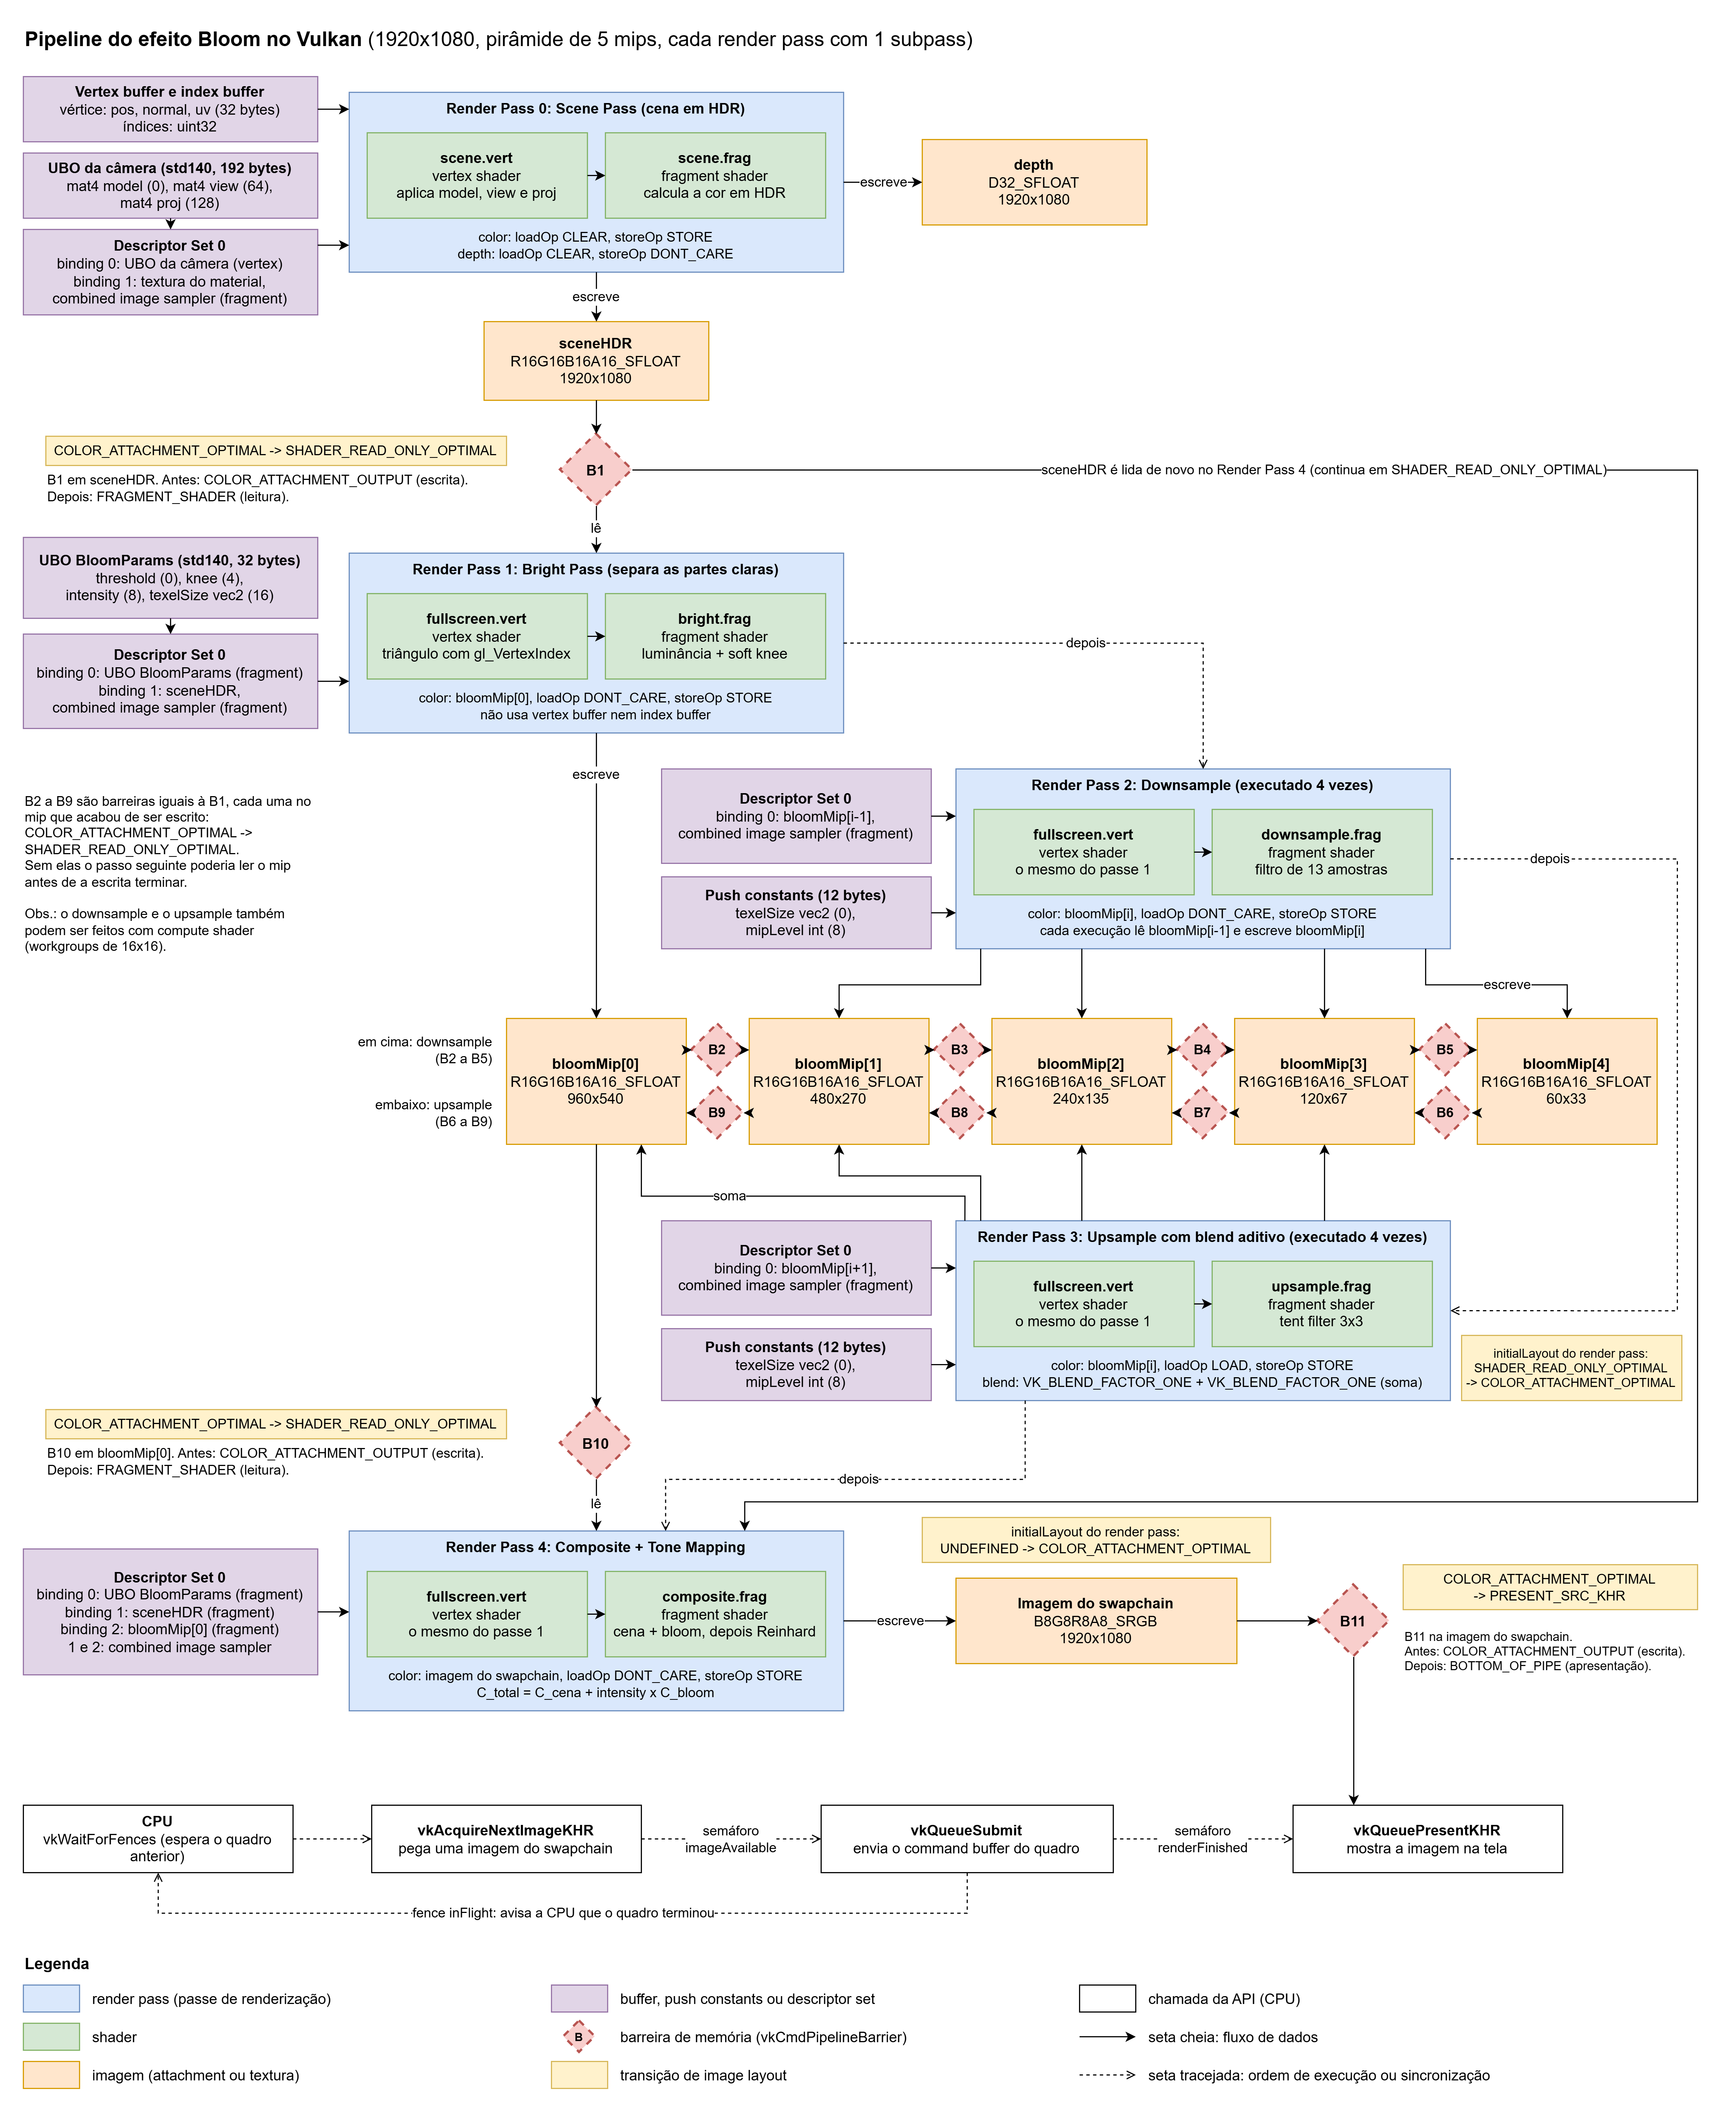
\includegraphics[height=0.64\textheight]{diagrama.png}
    \caption{Arquitetura do pipeline Vulkan para o efeito de \textit{Bloom}. Azul: \textit{render pass}. Verde: \textit{shader}. Laranja: imagem. Roxo: \textit{buffer} ou \textit{descriptor set}. Losango vermelho: barreira de memória. Amarelo: transição de \textit{layout}. Seta cheia: dados. Seta tracejada: ordem de execução ou sincronização.}
    \label{fig:pipeline}
\end{figure}

\subsection{Fluxo de Dados}
O quadro é desenhado em onze passes, gravados em ordem em um único \textit{command buffer}:
\begin{enumerate}
    \setlength{\itemsep}{0pt}
    \item \textbf{Passe 0 (\textit{Scene Pass}):} recebe o \textit{vertex buffer}, o \textit{index buffer}, o UBO da câmera e as texturas. Desenha a cena na \texttt{sceneHDR}, usando a \texttt{depth} no teste de profundidade.
    \item \textbf{Passe 1 (\textit{Bright Pass}):} lê a \texttt{sceneHDR} e guarda só as partes claras na \texttt{bloomMip[0]}, com metade da resolução.
    \item \textbf{Passes 2 a 5 (\textit{Downsample}):} cada execução lê \texttt{bloomMip[i-1]} e escreve \texttt{bloomMip[i]}, menor e mais borrado.
    \item \textbf{Passes 6 a 9 (\textit{Upsample}):} cada execução lê \texttt{bloomMip[i+1]} e soma o resultado em \texttt{bloomMip[i]}. No fim, a \texttt{bloomMip[0]} tem o halo completo.
    \item \textbf{Passe 10 (\textit{Composite}):} soma a \texttt{sceneHDR} com a \texttt{bloomMip[0]}, aplica o \textit{tone mapping} e escreve na imagem do \textit{swapchain}, que é mostrada na tela.
\end{enumerate}
\textbf{Recursos compartilhados.} A \texttt{sceneHDR} é lida nos passes 1 e 10. Os níveis \texttt{bloomMip} são \textit{mip levels} de uma mesma \texttt{VkImage}, usados na descida e na subida. O UBO \texttt{BloomParams} serve aos passes 1 e 10, e o \texttt{fullscreen.vert} e o \texttt{VkSampler} são os mesmos em todos os passes de tela cheia.

\subsection{Render Passes e Subpasses}
São cinco \textit{render passes}, todos com um único \textit{subpass} (Tabela~\ref{tab:renderpasses}).

\begin{table}[H]
    \centering
    \caption{\textit{Render passes} do pipeline.}
    \label{tab:renderpasses}
    \vspace{4pt}
    \scriptsize
    \setlength{\tabcolsep}{4pt}
    \begin{tabular}{c c l l l l}
        \toprule
        \textbf{RP} & \textbf{Passes} & \textbf{Attachment} & \textbf{loadOp / storeOp} & \textbf{initialLayout} & \textbf{Resultado} \\
        \midrule
        0 & 0 & \texttt{sceneHDR} (cor) & \texttt{CLEAR / STORE} & \texttt{UNDEFINED} & cena em HDR \\
          &   & \texttt{depth} (profundidade) & \texttt{CLEAR / DONT\_CARE} & \texttt{UNDEFINED} & teste de profundidade \\
        1 & 1 & \texttt{bloomMip[0]} & \texttt{DONT\_CARE / STORE} & \texttt{UNDEFINED} & partes claras da cena \\
        2 & 2 a 5 & \texttt{bloomMip[1]} a \texttt{bloomMip[4]} & \texttt{DONT\_CARE / STORE} & \texttt{UNDEFINED} & nível menor e borrado \\
        3 & 6 a 9 & \texttt{bloomMip[3]} a \texttt{bloomMip[0]} & \texttt{LOAD / STORE} & \texttt{SHADER\_READ\_ONLY\_OPTIMAL} & soma dos níveis \\
        4 & 10 & imagem do \textit{swapchain} & \texttt{DONT\_CARE / STORE} & \texttt{UNDEFINED} & imagem final \\
        \bottomrule
    \end{tabular}
\end{table}

No início do \textit{subpass}, o \textit{render pass} leva o \textit{attachment} do \texttt{initialLayout} para \texttt{COLOR\_ATTACHMENT\_OPTIMAL}. O \textit{upsample} usa \texttt{LOAD} porque precisa manter o conteúdo anterior para a soma. Os passes ficaram em \textit{render passes} separados porque cada um escreve em uma imagem de tamanho diferente e lê \textit{texels} vizinhos da anterior com um \textit{sampler}, o que um \textit{input attachment} não permite. O \texttt{VK\_KHR\_dynamic\_rendering} não foi usado por não ser o modelo visto na disciplina.

\subsection{Descriptor Sets e Bindings}
Todos os pipelines usam só o \textit{set} 0 (Tabela~\ref{tab:descriptors}). No \textit{downsample} e no \textit{upsample} há um \textit{descriptor set} para cada nível lido.

\begin{table}[H]
    \centering
    \caption{\textit{Descriptor sets} e \textit{bindings} de cada passe.}
    \label{tab:descriptors}
    \vspace{4pt}
    \scriptsize
    \setlength{\tabcolsep}{5pt}
    \begin{tabular}{l c c l l l}
        \toprule
        \textbf{Passe} & \textbf{Set} & \textbf{Binding} & \textbf{Tipo} & \textbf{Recurso} & \textbf{Estágio} \\
        \midrule
        0 (\textit{Scene}) & 0 & 0 & \texttt{UNIFORM\_BUFFER} & UBO da câmera & \textit{vertex} \\
                           & 0 & 1 & \texttt{COMBINED\_IMAGE\_SAMPLER} & textura do material & \textit{fragment} \\
        1 (\textit{Bright}) & 0 & 0 & \texttt{UNIFORM\_BUFFER} & \texttt{BloomParams} & \textit{fragment} \\
                            & 0 & 1 & \texttt{COMBINED\_IMAGE\_SAMPLER} & \texttt{sceneHDR} & \textit{fragment} \\
        2 a 5 (\textit{Downsample}) & 0 & 0 & \texttt{COMBINED\_IMAGE\_SAMPLER} & \texttt{bloomMip[i-1]} & \textit{fragment} \\
        6 a 9 (\textit{Upsample}) & 0 & 0 & \texttt{COMBINED\_IMAGE\_SAMPLER} & \texttt{bloomMip[i+1]} & \textit{fragment} \\
        10 (\textit{Composite}) & 0 & 0 & \texttt{UNIFORM\_BUFFER} & \texttt{BloomParams} & \textit{fragment} \\
                                & 0 & 1 & \texttt{COMBINED\_IMAGE\_SAMPLER} & \texttt{sceneHDR} & \textit{fragment} \\
                                & 0 & 2 & \texttt{COMBINED\_IMAGE\_SAMPLER} & \texttt{bloomMip[0]} & \textit{fragment} \\
        \bottomrule
    \end{tabular}
\end{table}

\subsection{Layout e Finalidade dos Buffers}
\begin{itemize}
    \setlength{\itemsep}{0pt}
    \item \textbf{\textit{Vertex buffer} e \textit{index buffer}:} geometria da cena, só no passe 0. Cada vértice tem 32 bytes: posição (\textit{offset} 0), normal (12) e coordenada de textura (24). Os índices são \texttt{uint32}.
    \item \textbf{UBO da câmera} (\texttt{std140}, 192 bytes): matrizes \texttt{model} (0), \texttt{view} (64) e \texttt{proj} (128).
    \item \textbf{UBO \texttt{BloomParams}} (\texttt{std140}, 32 bytes): \texttt{threshold} (0), \texttt{knee} (4), \texttt{intensity} (8) e \texttt{texelSize} (16), que são os parâmetros das Equações~\ref{eq:softknee} e~\ref{eq:reinhard}.
    \item \textbf{\textit{Push constants}} (12 bytes): \texttt{texelSize} (0) e \texttt{mipLevel} (8), que mudam a cada execução do \textit{downsample} e do \textit{upsample}.
\end{itemize}
Os passes 1 a 10 não têm \textit{vertex buffer}: o \texttt{fullscreen.vert} gera o triângulo de tela cheia a partir do \texttt{gl\_VertexIndex}, desenhado com \texttt{vkCmdDraw(3, 1, 0, 0)}.

\subsection{Shaders Envolvidos}
O pipeline usa apenas \textit{vertex} e \textit{fragment shaders}:
\begin{itemize}
    \setlength{\itemsep}{0pt}
    \item \texttt{scene.vert} e \texttt{scene.frag}: transformam os vértices e calculam a cor em HDR, que pode passar de $1.0$. Nos passes 1 a 10 o \textit{vertex shader} é sempre o \texttt{fullscreen.vert}.
    \item \texttt{bright.frag}: luminância (Equação~\ref{eq:luminancia}) e corte com joelho suave (Equação~\ref{eq:softknee}).
    \item \texttt{downsample.frag}: média de 13 amostras que reduz e borra, no papel do filtro da Equação~\ref{eq:gauss}.
    \item \texttt{upsample.frag}: \textit{tent filter} $3 \times 3$. A soma é feita pelo \textit{blend} aditivo, com \texttt{VK\_BLEND\_FACTOR\_ONE} na origem e no destino.
    \item \texttt{composite.frag}: soma a cena com o \textit{Bloom} e aplica o \textit{tone mapping} de Reinhard (Equação~\ref{eq:reinhard}) \cite{reinhard2002tone}.
\end{itemize}

\subsection{Barreiras de Memória e Transições de Layout}
\label{sec:barreiras}
A GPU pode começar a ler uma imagem antes de a escrita terminar. Além disso, o \textit{attachment} fica em \texttt{COLOR\_ATTACHMENT\_OPTIMAL} e a leitura por \textit{sampler} exige \texttt{SHADER\_READ\_ONLY\_OPTIMAL}. Por isso há uma barreira (\texttt{vkCmdPipelineBarrier}) sempre que uma imagem escrita em um passe é lida no seguinte (Tabela~\ref{tab:barreiras}).

\begin{table}[H]
    \centering
    \caption{As 11 barreiras de memória do diagrama.}
    \label{tab:barreiras}
    \vspace{4pt}
    \scriptsize
    \begin{tabular}{l l l @{\hspace{0.9cm}} l l l}
        \toprule
        & \textbf{Imagem} & \textbf{Escrita $\to$ leitura} & & \textbf{Imagem} & \textbf{Escrita $\to$ leitura} \\
        \midrule
        B1 & \texttt{sceneHDR} & passe 0 $\to$ passes 1 e 10 & B7 & \texttt{bloomMip[3]} & passe 6 $\to$ passe 7 \\
        B2 & \texttt{bloomMip[0]} & passe 1 $\to$ passe 2 & B8 & \texttt{bloomMip[2]} & passe 7 $\to$ passe 8 \\
        B3 & \texttt{bloomMip[1]} & passe 2 $\to$ passe 3 & B9 & \texttt{bloomMip[1]} & passe 8 $\to$ passe 9 \\
        B4 & \texttt{bloomMip[2]} & passe 3 $\to$ passe 4 & B10 & \texttt{bloomMip[0]} & passe 9 $\to$ passe 10 \\
        B5 & \texttt{bloomMip[3]} & passe 4 $\to$ passe 5 & B11 & \textit{swapchain} & passe 10 $\to$ apresentação \\
        B6 & \texttt{bloomMip[4]} & passe 5 $\to$ passe 6 & & & \\
        \bottomrule
    \end{tabular}
\end{table}

Nas barreiras B1 a B10 os dados são os mesmos: o acesso anterior é uma escrita (\texttt{COLOR\_ATTACHMENT\_WRITE}) no estágio \texttt{COLOR\_ATTACHMENT\_OUTPUT}, o acesso posterior é uma leitura (\texttt{SHADER\_READ}) no estágio \texttt{FRAGMENT\_SHADER} e o \textit{layout} muda de \texttt{COLOR\_ATTACHMENT\_OPTIMAL} para \texttt{SHADER\_READ\_ONLY\_OPTIMAL}. Na B11 o acesso anterior é o mesmo, depois não há outro acesso da GPU (estágio \texttt{BOTTOM\_OF\_PIPE}) e o \textit{layout} vira \texttt{PRESENT\_SRC\_KHR}, exigido para a apresentação. O motivo é igual em todas: a imagem só pode ser usada depois que a escrita terminou e ela está no \textit{layout} certo.

As outras transições de \textit{layout} são feitas pelos \textit{render passes} com o \texttt{initialLayout} e aparecem em amarelo no diagrama. A \texttt{sceneHDR} é lida de novo no passe 10 sem outra barreira, porque continua no \textit{layout} de leitura. A sincronização entre CPU e GPU usa os semáforos \texttt{imageAvailable} e \texttt{renderFinished} e a \textit{fence} \texttt{inFlight}, mostrados na parte de baixo do diagrama.

\subsection{Justificativa das Decisões}
\begin{itemize}
    \setlength{\itemsep}{0pt}
    \item \textbf{Triângulo de tela cheia:} dispensa \textit{vertex buffer} e evita a diagonal que um \textit{quad} teria (Seção~\ref{sec:vulkan}).
    \item \textbf{Pirâmide de \textit{mips}:} um borrão largo feito de uma vez em resolução cheia precisaria de muitas amostras por pixel (Equação~\ref{eq:gauss}). Com a imagem reduzida pela metade a cada nível, um filtro pequeno alcança um raio grande, e a soma dos níveis lembra o espalhamento de Spencer et al. \cite{spencer1995glare}.
    \item \textbf{Formato de 16 bits em ponto flutuante:} guarda valores acima de $1.0$, que diferenciam uma luz forte de uma superfície branca \cite{seetzen2004hdr}. Com 8 bits eles seriam cortados.
    \item \textbf{\textit{Fragment shader} em vez de \textit{compute shader}:} a Seção~\ref{sec:vulkan} cita que o borrão também pode usar \textit{compute shaders} em \textit{workgroups} de $16 \times 16$. O grupo desenhou a versão com \textit{fragment shader} por ser mais simples: todos os passes têm a mesma estrutura e as barreiras são iguais. Com \textit{compute}, o destino seria uma \texttt{STORAGE\_IMAGE} no \textit{layout} \texttt{GENERAL} e as barreiras usariam o estágio \texttt{COMPUTE\_SHADER}.
\end{itemize}
\textbf{Relação com a técnica.} O desenho segue as quatro fases da Seção~\ref{sec:funciona}: \textit{bright pass} (passe 1), \textit{downsampling} (passes 2 a 5), \textit{upsampling} com soma (passes 6 a 9) e composição com \textit{tone mapping} (passe 10). Os recursos também são próprios do \textit{Bloom}: a \texttt{sceneHDR} em ponto flutuante, a pirâmide \texttt{bloomMip}, o \textit{blend} aditivo e o UBO com o limiar e a intensidade.
\fussy

% ===============================================================

\section{Arquitetura do Pipeline Vulkan}
\label{sec:arquitetura}
\sloppy

Esta seção é a segunda entrega do trabalho. A Figura~\ref{fig:pipeline} mostra o desenho do pipeline Vulkan que executa o \textit{Bloom}, feito no draw.io. Como exemplo, o grupo considerou uma tela de $1920 \times 1080$, imagens no formato \texttt{VK\_FORMAT\_R16G16B16A16\_SFLOAT}, citado na Seção~\ref{sec:vulkan}, e uma pirâmide de cinco níveis, de \texttt{bloomMip[0]} a \texttt{bloomMip[4]}.

\begin{figure}[H]
    \centering
    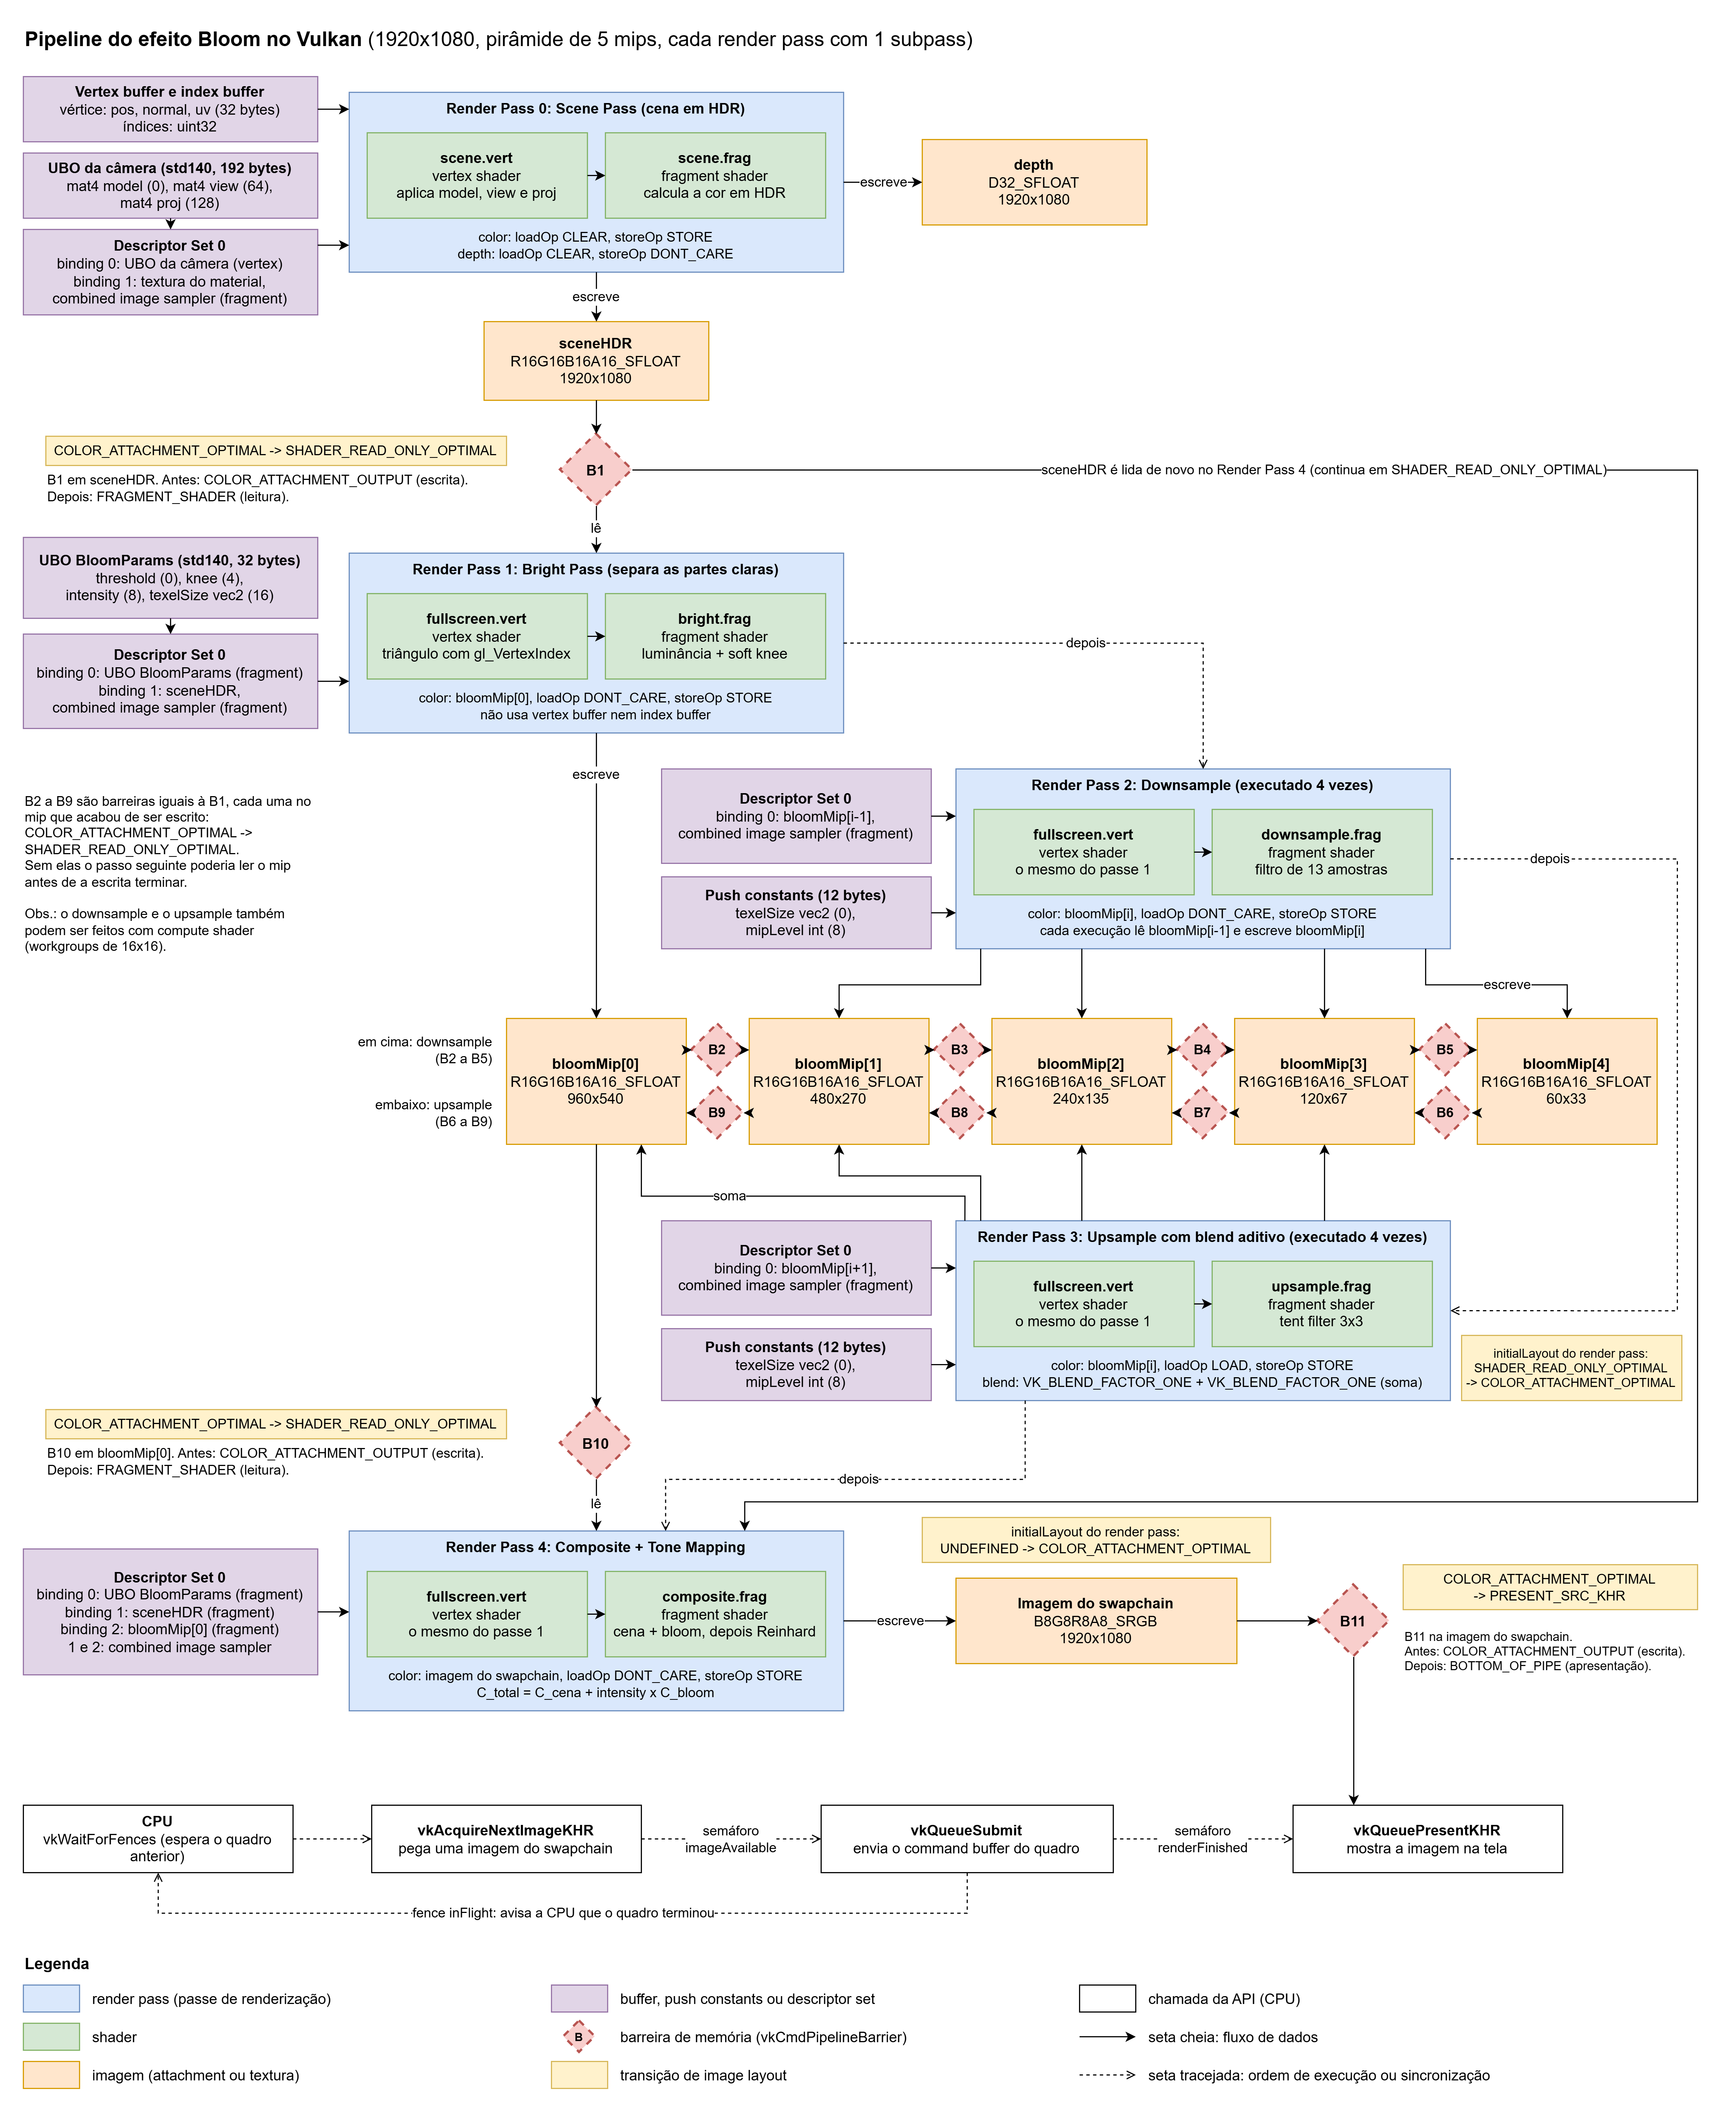
\includegraphics[height=0.64\textheight]{diagrama.png}
    \caption{Arquitetura do pipeline Vulkan para o efeito de \textit{Bloom}. Azul: \textit{render pass}. Verde: \textit{shader}. Laranja: imagem. Roxo: \textit{buffer} ou \textit{descriptor set}. Losango vermelho: barreira de memória. Amarelo: transição de \textit{layout}. Seta cheia: dados. Seta tracejada: ordem de execução ou sincronização.}
    \label{fig:pipeline}
\end{figure}

\subsection{Fluxo de Dados}
O quadro é desenhado em onze passes, gravados em ordem em um único \textit{command buffer}:
\begin{enumerate}
    \setlength{\itemsep}{0pt}
    \item \textbf{Passe 0 (\textit{Scene Pass}):} recebe o \textit{vertex buffer}, o \textit{index buffer}, o UBO da câmera e as texturas. Desenha a cena na \texttt{sceneHDR}, usando a \texttt{depth} no teste de profundidade.
    \item \textbf{Passe 1 (\textit{Bright Pass}):} lê a \texttt{sceneHDR} e guarda só as partes claras na \texttt{bloomMip[0]}, com metade da resolução.
    \item \textbf{Passes 2 a 5 (\textit{Downsample}):} cada execução lê \texttt{bloomMip[i-1]} e escreve \texttt{bloomMip[i]}, menor e mais borrado.
    \item \textbf{Passes 6 a 9 (\textit{Upsample}):} cada execução lê \texttt{bloomMip[i+1]} e soma o resultado em \texttt{bloomMip[i]}. No fim, a \texttt{bloomMip[0]} tem o halo completo.
    \item \textbf{Passe 10 (\textit{Composite}):} soma a \texttt{sceneHDR} com a \texttt{bloomMip[0]}, aplica o \textit{tone mapping} e escreve na imagem do \textit{swapchain}, que é mostrada na tela.
\end{enumerate}
\textbf{Recursos compartilhados.} A \texttt{sceneHDR} é lida nos passes 1 e 10. Os níveis \texttt{bloomMip} são \textit{mip levels} de uma mesma \texttt{VkImage}, usados na descida e na subida. O UBO \texttt{BloomParams} serve aos passes 1 e 10, e o \texttt{fullscreen.vert} e o \texttt{VkSampler} são os mesmos em todos os passes de tela cheia.

\subsection{Render Passes e Subpasses}
São cinco \textit{render passes}, todos com um único \textit{subpass} (Tabela~\ref{tab:renderpasses}).

\begin{table}[H]
    \centering
    \caption{\textit{Render passes} do pipeline.}
    \label{tab:renderpasses}
    \vspace{4pt}
    \scriptsize
    \setlength{\tabcolsep}{4pt}
    \begin{tabular}{c c l l l l}
        \toprule
        \textbf{RP} & \textbf{Passes} & \textbf{Attachment} & \textbf{loadOp / storeOp} & \textbf{initialLayout} & \textbf{Resultado} \\
        \midrule
        0 & 0 & \texttt{sceneHDR} (cor) & \texttt{CLEAR / STORE} & \texttt{UNDEFINED} & cena em HDR \\
          &   & \texttt{depth} (profundidade) & \texttt{CLEAR / DONT\_CARE} & \texttt{UNDEFINED} & teste de profundidade \\
        1 & 1 & \texttt{bloomMip[0]} & \texttt{DONT\_CARE / STORE} & \texttt{UNDEFINED} & partes claras da cena \\
        2 & 2 a 5 & \texttt{bloomMip[1]} a \texttt{bloomMip[4]} & \texttt{DONT\_CARE / STORE} & \texttt{UNDEFINED} & nível menor e borrado \\
        3 & 6 a 9 & \texttt{bloomMip[3]} a \texttt{bloomMip[0]} & \texttt{LOAD / STORE} & \texttt{SHADER\_READ\_ONLY\_OPTIMAL} & soma dos níveis \\
        4 & 10 & imagem do \textit{swapchain} & \texttt{DONT\_CARE / STORE} & \texttt{UNDEFINED} & imagem final \\
        \bottomrule
    \end{tabular}
\end{table}

No início do \textit{subpass}, o \textit{render pass} leva o \textit{attachment} do \texttt{initialLayout} para \texttt{COLOR\_ATTACHMENT\_OPTIMAL}. O \textit{upsample} usa \texttt{LOAD} porque precisa manter o conteúdo anterior para a soma. Os passes ficaram em \textit{render passes} separados porque cada um escreve em uma imagem de tamanho diferente e lê \textit{texels} vizinhos da anterior com um \textit{sampler}, o que um \textit{input attachment} não permite. O \texttt{VK\_KHR\_dynamic\_rendering} não foi usado por não ser o modelo visto na disciplina.

\subsection{Descriptor Sets e Bindings}
Todos os pipelines usam só o \textit{set} 0 (Tabela~\ref{tab:descriptors}). No \textit{downsample} e no \textit{upsample} há um \textit{descriptor set} para cada nível lido.

\begin{table}[H]
    \centering
    \caption{\textit{Descriptor sets} e \textit{bindings} de cada passe.}
    \label{tab:descriptors}
    \vspace{4pt}
    \scriptsize
    \setlength{\tabcolsep}{5pt}
    \begin{tabular}{l c c l l l}
        \toprule
        \textbf{Passe} & \textbf{Set} & \textbf{Binding} & \textbf{Tipo} & \textbf{Recurso} & \textbf{Estágio} \\
        \midrule
        0 (\textit{Scene}) & 0 & 0 & \texttt{UNIFORM\_BUFFER} & UBO da câmera & \textit{vertex} \\
                           & 0 & 1 & \texttt{COMBINED\_IMAGE\_SAMPLER} & textura do material & \textit{fragment} \\
        1 (\textit{Bright}) & 0 & 0 & \texttt{UNIFORM\_BUFFER} & \texttt{BloomParams} & \textit{fragment} \\
                            & 0 & 1 & \texttt{COMBINED\_IMAGE\_SAMPLER} & \texttt{sceneHDR} & \textit{fragment} \\
        2 a 5 (\textit{Downsample}) & 0 & 0 & \texttt{COMBINED\_IMAGE\_SAMPLER} & \texttt{bloomMip[i-1]} & \textit{fragment} \\
        6 a 9 (\textit{Upsample}) & 0 & 0 & \texttt{COMBINED\_IMAGE\_SAMPLER} & \texttt{bloomMip[i+1]} & \textit{fragment} \\
        10 (\textit{Composite}) & 0 & 0 & \texttt{UNIFORM\_BUFFER} & \texttt{BloomParams} & \textit{fragment} \\
                                & 0 & 1 & \texttt{COMBINED\_IMAGE\_SAMPLER} & \texttt{sceneHDR} & \textit{fragment} \\
                                & 0 & 2 & \texttt{COMBINED\_IMAGE\_SAMPLER} & \texttt{bloomMip[0]} & \textit{fragment} \\
        \bottomrule
    \end{tabular}
\end{table}

\subsection{Layout e Finalidade dos Buffers}
\begin{itemize}
    \setlength{\itemsep}{0pt}
    \item \textbf{\textit{Vertex buffer} e \textit{index buffer}:} geometria da cena, só no passe 0. Cada vértice tem 32 bytes: posição (\textit{offset} 0), normal (12) e coordenada de textura (24). Os índices são \texttt{uint32}.
    \item \textbf{UBO da câmera} (\texttt{std140}, 192 bytes): matrizes \texttt{model} (0), \texttt{view} (64) e \texttt{proj} (128).
    \item \textbf{UBO \texttt{BloomParams}} (\texttt{std140}, 32 bytes): \texttt{threshold} (0), \texttt{knee} (4), \texttt{intensity} (8) e \texttt{texelSize} (16), que são os parâmetros das Equações~\ref{eq:softknee} e~\ref{eq:reinhard}.
    \item \textbf{\textit{Push constants}} (12 bytes): \texttt{texelSize} (0) e \texttt{mipLevel} (8), que mudam a cada execução do \textit{downsample} e do \textit{upsample}.
\end{itemize}
Os passes 1 a 10 não têm \textit{vertex buffer}: o \texttt{fullscreen.vert} gera o triângulo de tela cheia a partir do \texttt{gl\_VertexIndex}, desenhado com \texttt{vkCmdDraw(3, 1, 0, 0)}.

\subsection{Shaders Envolvidos}
O pipeline usa apenas \textit{vertex} e \textit{fragment shaders}:
\begin{itemize}
    \setlength{\itemsep}{0pt}
    \item \texttt{scene.vert} e \texttt{scene.frag}: transformam os vértices e calculam a cor em HDR, que pode passar de $1.0$. Nos passes 1 a 10 o \textit{vertex shader} é sempre o \texttt{fullscreen.vert}.
    \item \texttt{bright.frag}: luminância (Equação~\ref{eq:luminancia}) e corte com joelho suave (Equação~\ref{eq:softknee}).
    \item \texttt{downsample.frag}: média de 13 amostras que reduz e borra, no papel do filtro da Equação~\ref{eq:gauss}.
    \item \texttt{upsample.frag}: \textit{tent filter} $3 \times 3$. A soma é feita pelo \textit{blend} aditivo, com \texttt{VK\_BLEND\_FACTOR\_ONE} na origem e no destino.
    \item \texttt{composite.frag}: soma a cena com o \textit{Bloom} e aplica o \textit{tone mapping} de Reinhard (Equação~\ref{eq:reinhard}) \cite{reinhard2002tone}.
\end{itemize}

\subsection{Barreiras de Memória e Transições de Layout}
\label{sec:barreiras}
A GPU pode começar a ler uma imagem antes de a escrita terminar. Além disso, o \textit{attachment} fica em \texttt{COLOR\_ATTACHMENT\_OPTIMAL} e a leitura por \textit{sampler} exige \texttt{SHADER\_READ\_ONLY\_OPTIMAL}. Por isso há uma barreira (\texttt{vkCmdPipelineBarrier}) sempre que uma imagem escrita em um passe é lida no seguinte (Tabela~\ref{tab:barreiras}).

\begin{table}[H]
    \centering
    \caption{As 11 barreiras de memória do diagrama.}
    \label{tab:barreiras}
    \vspace{4pt}
    \scriptsize
    \begin{tabular}{l l l @{\hspace{0.9cm}} l l l}
        \toprule
        & \textbf{Imagem} & \textbf{Escrita $\to$ leitura} & & \textbf{Imagem} & \textbf{Escrita $\to$ leitura} \\
        \midrule
        B1 & \texttt{sceneHDR} & passe 0 $\to$ passes 1 e 10 & B7 & \texttt{bloomMip[3]} & passe 6 $\to$ passe 7 \\
        B2 & \texttt{bloomMip[0]} & passe 1 $\to$ passe 2 & B8 & \texttt{bloomMip[2]} & passe 7 $\to$ passe 8 \\
        B3 & \texttt{bloomMip[1]} & passe 2 $\to$ passe 3 & B9 & \texttt{bloomMip[1]} & passe 8 $\to$ passe 9 \\
        B4 & \texttt{bloomMip[2]} & passe 3 $\to$ passe 4 & B10 & \texttt{bloomMip[0]} & passe 9 $\to$ passe 10 \\
        B5 & \texttt{bloomMip[3]} & passe 4 $\to$ passe 5 & B11 & \textit{swapchain} & passe 10 $\to$ apresentação \\
        B6 & \texttt{bloomMip[4]} & passe 5 $\to$ passe 6 & & & \\
        \bottomrule
    \end{tabular}
\end{table}

Nas barreiras B1 a B10 os dados são os mesmos: o acesso anterior é uma escrita (\texttt{COLOR\_ATTACHMENT\_WRITE}) no estágio \texttt{COLOR\_ATTACHMENT\_OUTPUT}, o acesso posterior é uma leitura (\texttt{SHADER\_READ}) no estágio \texttt{FRAGMENT\_SHADER} e o \textit{layout} muda de \texttt{COLOR\_ATTACHMENT\_OPTIMAL} para \texttt{SHADER\_READ\_ONLY\_OPTIMAL}. Na B11 o acesso anterior é o mesmo, depois não há outro acesso da GPU (estágio \texttt{BOTTOM\_OF\_PIPE}) e o \textit{layout} vira \texttt{PRESENT\_SRC\_KHR}, exigido para a apresentação. O motivo é igual em todas: a imagem só pode ser usada depois que a escrita terminou e ela está no \textit{layout} certo.

As outras transições de \textit{layout} são feitas pelos \textit{render passes} com o \texttt{initialLayout} e aparecem em amarelo no diagrama. A \texttt{sceneHDR} é lida de novo no passe 10 sem outra barreira, porque continua no \textit{layout} de leitura. A sincronização entre CPU e GPU usa os semáforos \texttt{imageAvailable} e \texttt{renderFinished} e a \textit{fence} \texttt{inFlight}, mostrados na parte de baixo do diagrama.

\subsection{Justificativa das Decisões}
\begin{itemize}
    \setlength{\itemsep}{0pt}
    \item \textbf{Triângulo de tela cheia:} dispensa \textit{vertex buffer} e evita a diagonal que um \textit{quad} teria (Seção~\ref{sec:vulkan}).
    \item \textbf{Pirâmide de \textit{mips}:} um borrão largo feito de uma vez em resolução cheia precisaria de muitas amostras por pixel (Equação~\ref{eq:gauss}). Com a imagem reduzida pela metade a cada nível, um filtro pequeno alcança um raio grande, e a soma dos níveis lembra o espalhamento de Spencer et al. \cite{spencer1995glare}.
    \item \textbf{Formato de 16 bits em ponto flutuante:} guarda valores acima de $1.0$, que diferenciam uma luz forte de uma superfície branca \cite{seetzen2004hdr}. Com 8 bits eles seriam cortados.
    \item \textbf{\textit{Fragment shader} em vez de \textit{compute shader}:} a Seção~\ref{sec:vulkan} cita que o borrão também pode usar \textit{compute shaders} em \textit{workgroups} de $16 \times 16$. O grupo desenhou a versão com \textit{fragment shader} por ser mais simples: todos os passes têm a mesma estrutura e as barreiras são iguais. Com \textit{compute}, o destino seria uma \texttt{STORAGE\_IMAGE} no \textit{layout} \texttt{GENERAL} e as barreiras usariam o estágio \texttt{COMPUTE\_SHADER}.
\end{itemize}
\textbf{Relação com a técnica.} O desenho segue as quatro fases da Seção~\ref{sec:funciona}: \textit{bright pass} (passe 1), \textit{downsampling} (passes 2 a 5), \textit{upsampling} com soma (passes 6 a 9) e composição com \textit{tone mapping} (passe 10). Os recursos também são próprios do \textit{Bloom}: a \texttt{sceneHDR} em ponto flutuante, a pirâmide \texttt{bloomMip}, o \textit{blend} aditivo e o UBO com o limiar e a intensidade.
\fussy


% Entrega 3: pseudocódigo dos shaders (GLSL)
% ===============================================================
% Entrega 3: Pseudocodigo dos shaders (GLSL)
% Incluido no main.tex com % ===============================================================
% Entrega 3: Pseudocodigo dos shaders (GLSL)
% Incluido no main.tex com % ===============================================================
% Entrega 3: Pseudocodigo dos shaders (GLSL)
% Incluido no main.tex com \input{entrega3}
% Os arquivos .vert e .frag ficam na pasta shaders/
% ===============================================================

% configuracao do pacote listings para mostrar os shaders
\lstset{
    language=C,
    morekeywords={vec2,vec3,vec4,mat3,mat4,sampler2D,uniform,layout,in,out,location,set,binding,push_constant},
    basicstyle=\linespread{1.0}\footnotesize\ttfamily,
    keywordstyle=\color{blue},
    commentstyle=\color{gray}\itshape,
    numbers=left,
    numberstyle=\tiny\color{gray},
    frame=single,
    breaklines=true,
    tabsize=4,
    showstringspaces=false,
    columns=fullflexible,
    keepspaces=true,
}
\renewcommand{\lstlistingname}{Código}

\section{Pseudocódigo dos Shaders}
\label{sec:pseudocodigo}
\sloppy

Nesta entrega escrevemos o pseudocódigo dos sete \textit{shaders} do pipeline da Entrega 2 (Seção~\ref{sec:arquitetura}). Os arquivos estão na pasta \texttt{shaders/} do \texttt{.zip}: dois \texttt{.vert} e cinco \texttt{.frag}. Não usamos \textit{compute shader}, então não há \texttt{.comp}. A sintaxe é a do GLSL do Vulkan (\texttt{\#version 450}), mas o código ainda não foi ligado a uma aplicação. Nos comentários, ``eq.~1'' a ``eq.~5'' são as equações da Seção~\ref{sec:equacoes}.

\subsection{Objetivo de Cada Shader}

\begin{table}[htb]
    \centering
    \caption{Os \textit{shaders} da entrega.}
    \label{tab:shaders}
    \vspace{4pt}
    \small
    \begin{tabular}{l l c p{7.2cm}}
        \toprule
        \textbf{Arquivo} & \textbf{Tipo} & \textbf{Passe} & \textbf{O que faz} \\
        \midrule
        \texttt{scene.vert} & \textit{vertex} & 0 & transforma os vértices da cena para a tela \\
        \texttt{scene.frag} & \textit{fragment} & 0 & calcula a cor da cena em HDR (sem limitar em 1.0) \\
        \texttt{fullscreen.vert} & \textit{vertex} & 1 a 10 & gera o triângulo de tela cheia dos passes de pós-processamento \\
        \texttt{bright.frag} & \textit{fragment} & 1 & deixa passar só as partes claras da cena (\textit{bright pass}) \\
        \texttt{downsample.frag} & \textit{fragment} & 2 a 5 & reduz a imagem pela metade e borra \\
        \texttt{upsample.frag} & \textit{fragment} & 6 a 9 & amplia o nível menor e soma no maior \\
        \texttt{composite.frag} & \textit{fragment} & 10 & soma cena e \textit{bloom} e faz o \textit{tone mapping} \\
        \bottomrule
    \end{tabular}
\end{table}

\subsection{Fluxo entre os Shaders}
O fluxo é o da Figura~\ref{fig:pipeline}: o \textit{fragment shader} de um passe escreve em uma imagem e o do passe seguinte lê essa imagem como textura, depois da barreira correspondente (Seção~\ref{sec:barreiras}).
\begin{center}
    \texttt{scene.vert} $\to$ \texttt{scene.frag} $\to$ \texttt{sceneHDR} $\to$ \texttt{bright.frag} $\to$ \texttt{bloomMip[0]} $\to$ \texttt{downsample.frag} (4 vezes) $\to$ \texttt{bloomMip[4]} $\to$ \texttt{upsample.frag} (4 vezes) $\to$ \texttt{bloomMip[0]} $\to$ \texttt{composite.frag} $\to$ \textit{swapchain}
\end{center}
Nos passes 1 a 10 o \textit{vertex shader} é sempre o \texttt{fullscreen.vert}. O \texttt{downsample.frag} e o \texttt{upsample.frag} rodam quatro vezes cada um, trocando a textura lida e os \textit{push constants}.

\subsection{Pseudocódigo Completo}

\lstinputlisting[caption={\texttt{scene.vert}}, label={lst:scenevert}]{shaders/scene.vert}
\lstinputlisting[caption={\texttt{scene.frag}}, label={lst:scenefrag}]{shaders/scene.frag}
\lstinputlisting[caption={\texttt{fullscreen.vert}}, label={lst:fullscreen}]{shaders/fullscreen.vert}
\lstinputlisting[caption={\texttt{bright.frag}}, label={lst:bright}]{shaders/bright.frag}
\lstinputlisting[caption={\texttt{downsample.frag}}, label={lst:downsample}]{shaders/downsample.frag}
\lstinputlisting[caption={\texttt{upsample.frag}}, label={lst:upsample}]{shaders/upsample.frag}
\lstinputlisting[caption={\texttt{composite.frag}}, label={lst:composite}]{shaders/composite.frag}

\subsection{Entradas e Saídas}
\begin{itemize}
    \setlength{\itemsep}{0pt}
    \item \texttt{scene.vert}: entram posição, normal e uv do \textit{vertex buffer} e as matrizes do UBO da câmera; saem \texttt{gl\_Position}, normal e uv.
    \item \texttt{scene.frag}: entram normal, uv e a textura do material; sai a cor HDR na \texttt{sceneHDR}.
    \item \texttt{fullscreen.vert}: entra só o \texttt{gl\_VertexIndex}; saem \texttt{gl\_Position} e o \texttt{uv}.
    \item \texttt{bright.frag}: entram \texttt{uv}, \texttt{sceneHDR} e o UBO \texttt{BloomParams}; sai a \texttt{bloomMip[0]}.
    \item \texttt{downsample.frag} e \texttt{upsample.frag}: entram \texttt{uv}, o nível lido e os \textit{push constants} (\texttt{texelSize} e \texttt{mipLevel}); sai o nível escrito (no \textit{upsample}, somado pelo \textit{blend}).
    \item \texttt{composite.frag}: entram \texttt{uv}, \texttt{sceneHDR}, \texttt{bloomMip[0]} e o \texttt{intensity}; sai a imagem final no \textit{swapchain}.
\end{itemize}
Os tipos (\texttt{vec2}, \texttt{vec3}, \texttt{mat4}, \texttt{sampler2D}) e os \textit{bindings} estão nas declarações de cada arquivo.

\subsection{Equações e Variáveis}
\begin{itemize}
    \setlength{\itemsep}{0pt}
    \item \texttt{scene.vert}: posição $= \mathbf{P}\,\mathbf{V}\,\mathbf{M}\,p$; a normal usa só a parte $3 \times 3$ da \texttt{model} e é normalizada de novo.
    \item \texttt{scene.frag}: difusa de Lambert, $\max(\mathbf{n} \cdot \mathbf{l}, 0)$, com luz de intensidade $4.0$ e emissivo $10.0$. Por isso a cena passa de $1.0$.
    \item \texttt{bright.frag}: \texttt{lum} é a Equação~\ref{eq:luminancia} e \texttt{peso} é a Equação~\ref{eq:softknee}, com \texttt{T} = \texttt{threshold}, \texttt{k} = \texttt{knee} e \texttt{EPS} = $\epsilon$. O peso vale $0$ até $L = T - k$ e fica em $k$ a partir de $L = T + k$.
    \item \texttt{downsample.frag}: 13 amostras com pesos $1/8$ (centro e internas), $1/16$ (bordas) e $1/32$ (cantos), que somam $1$.
    \item \texttt{upsample.frag}: filtro tenda $\frac{1}{16}\begin{bmatrix} 1 & 2 & 1 \\ 2 & 4 & 2 \\ 1 & 2 & 1 \end{bmatrix}$, que também soma $1$. Os dois filtros fazem o papel da Gaussiana da Equação~\ref{eq:gauss}: o borrão fica largo porque a imagem cai pela metade a cada nível.
    \item \texttt{composite.frag}: Equação~\ref{eq:reinhard}, \texttt{total} $= C_{\text{cena}} + \alpha\,C_{\text{bloom}}$ e \texttt{cor} $= \texttt{total}/(1 + \texttt{total})$. Uma luz de $10.0$ vira $0.91$ e uma parede branca de $1.0$ vira $0.5$.
\end{itemize}

\subsection{Loops e Condições}
O \texttt{bright.frag} tem um \texttt{for} de 4 iterações (uma por pixel do bloco $2 \times 2$) e o \texttt{upsample.frag} tem dois \texttt{for} aninhados de $-1$ a $1$ (9 amostras). No \texttt{downsample.frag} as 13 amostras estão escritas uma a uma, e o \texttt{if (pc.mipLevel == 1)} corta valores acima de $10.0$ só no primeiro nível, para pixels isolados não piscarem. Casos extremos: o \texttt{max} zera luz negativa (\texttt{scene.frag} e \texttt{bright.frag}), o \texttt{EPS} evita divisão por zero, o \texttt{clamp} do \texttt{composite.frag} garante o intervalo do \textit{swapchain} e o \texttt{CLAMP\_TO\_EDGE} do \textit{sampler} repete o pixel da borda em vez de ler fora da imagem.

\subsection{Amostragem de Texturas}
Todas as leituras usam \texttt{sampler2D} e \texttt{texture()}. A textura do material tem mipmaps e \textit{sampler} trilinear com \texttt{REPEAT}; o nível é escolhido pelo hardware. As imagens do \textit{bloom} têm um nível só (o \texttt{texture()} lê o nível 0), filtro \texttt{LINEAR} e \texttt{CLAMP\_TO\_EDGE}. O filtro linear faz a média dos vizinhos quando a amostra cai entre dois pixels (\texttt{bright} e \texttt{downsample}) e amplia a imagem menor sem serrilhado (\texttt{upsample} e \texttt{composite}). Os deslocamentos são múltiplos do \texttt{texelSize} da imagem lida.

\subsection{Resultado Esperado}
A \texttt{bloomMip[0]} sai do \textit{bright pass} quase toda preta, só com as luzes. Cada \textit{downsample} gera um nível menor e mais borrado, até $60 \times 33$, e cada \textit{upsample} soma o nível menor no maior; no fim a \texttt{bloomMip[0]} tem um halo largo e suave em volta de cada luz. O \texttt{composite.frag} soma esse halo na cena e comprime para $[0, 1]$: é a imagem final, com as luzes ``sangrando'' como nas Figuras~\ref{fig:portal} e~\ref{fig:cyberpunk}.

\subsection{Relação com a Técnica}
Os \textit{shaders} são as quatro fases da Seção~\ref{sec:funciona}: \textit{bright pass} (Equações~\ref{eq:luminancia} e~\ref{eq:softknee}), \textit{downsampling}, \textit{upsampling} com soma e \textit{tone mapping} (Equação~\ref{eq:reinhard}). A pirâmide substitui a Gaussiana grande da Equação~\ref{eq:gauss}, e a soma de borrões de vários tamanhos aproxima o espalhamento da Equação~\ref{eq:psf} \cite{spencer1995glare}. Cada arquivo corresponde a um passe e a um \textit{descriptor set} da Seção~\ref{sec:arquitetura}.
\fussy

% Os arquivos .vert e .frag ficam na pasta shaders/
% ===============================================================

% configuracao do pacote listings para mostrar os shaders
\lstset{
    language=C,
    morekeywords={vec2,vec3,vec4,mat3,mat4,sampler2D,uniform,layout,in,out,location,set,binding,push_constant},
    basicstyle=\linespread{1.0}\footnotesize\ttfamily,
    keywordstyle=\color{blue},
    commentstyle=\color{gray}\itshape,
    numbers=left,
    numberstyle=\tiny\color{gray},
    frame=single,
    breaklines=true,
    tabsize=4,
    showstringspaces=false,
    columns=fullflexible,
    keepspaces=true,
}
\renewcommand{\lstlistingname}{Código}

\section{Pseudocódigo dos Shaders}
\label{sec:pseudocodigo}
\sloppy

Nesta entrega escrevemos o pseudocódigo dos sete \textit{shaders} do pipeline da Entrega 2 (Seção~\ref{sec:arquitetura}). Os arquivos estão na pasta \texttt{shaders/} do \texttt{.zip}: dois \texttt{.vert} e cinco \texttt{.frag}. Não usamos \textit{compute shader}, então não há \texttt{.comp}. A sintaxe é a do GLSL do Vulkan (\texttt{\#version 450}), mas o código ainda não foi ligado a uma aplicação. Nos comentários, ``eq.~1'' a ``eq.~5'' são as equações da Seção~\ref{sec:equacoes}.

\subsection{Objetivo de Cada Shader}

\begin{table}[htb]
    \centering
    \caption{Os \textit{shaders} da entrega.}
    \label{tab:shaders}
    \vspace{4pt}
    \small
    \begin{tabular}{l l c p{7.2cm}}
        \toprule
        \textbf{Arquivo} & \textbf{Tipo} & \textbf{Passe} & \textbf{O que faz} \\
        \midrule
        \texttt{scene.vert} & \textit{vertex} & 0 & transforma os vértices da cena para a tela \\
        \texttt{scene.frag} & \textit{fragment} & 0 & calcula a cor da cena em HDR (sem limitar em 1.0) \\
        \texttt{fullscreen.vert} & \textit{vertex} & 1 a 10 & gera o triângulo de tela cheia dos passes de pós-processamento \\
        \texttt{bright.frag} & \textit{fragment} & 1 & deixa passar só as partes claras da cena (\textit{bright pass}) \\
        \texttt{downsample.frag} & \textit{fragment} & 2 a 5 & reduz a imagem pela metade e borra \\
        \texttt{upsample.frag} & \textit{fragment} & 6 a 9 & amplia o nível menor e soma no maior \\
        \texttt{composite.frag} & \textit{fragment} & 10 & soma cena e \textit{bloom} e faz o \textit{tone mapping} \\
        \bottomrule
    \end{tabular}
\end{table}

\subsection{Fluxo entre os Shaders}
O fluxo é o da Figura~\ref{fig:pipeline}: o \textit{fragment shader} de um passe escreve em uma imagem e o do passe seguinte lê essa imagem como textura, depois da barreira correspondente (Seção~\ref{sec:barreiras}).
\begin{center}
    \texttt{scene.vert} $\to$ \texttt{scene.frag} $\to$ \texttt{sceneHDR} $\to$ \texttt{bright.frag} $\to$ \texttt{bloomMip[0]} $\to$ \texttt{downsample.frag} (4 vezes) $\to$ \texttt{bloomMip[4]} $\to$ \texttt{upsample.frag} (4 vezes) $\to$ \texttt{bloomMip[0]} $\to$ \texttt{composite.frag} $\to$ \textit{swapchain}
\end{center}
Nos passes 1 a 10 o \textit{vertex shader} é sempre o \texttt{fullscreen.vert}. O \texttt{downsample.frag} e o \texttt{upsample.frag} rodam quatro vezes cada um, trocando a textura lida e os \textit{push constants}.

\subsection{Pseudocódigo Completo}

\lstinputlisting[caption={\texttt{scene.vert}}, label={lst:scenevert}]{shaders/scene.vert}
\lstinputlisting[caption={\texttt{scene.frag}}, label={lst:scenefrag}]{shaders/scene.frag}
\lstinputlisting[caption={\texttt{fullscreen.vert}}, label={lst:fullscreen}]{shaders/fullscreen.vert}
\lstinputlisting[caption={\texttt{bright.frag}}, label={lst:bright}]{shaders/bright.frag}
\lstinputlisting[caption={\texttt{downsample.frag}}, label={lst:downsample}]{shaders/downsample.frag}
\lstinputlisting[caption={\texttt{upsample.frag}}, label={lst:upsample}]{shaders/upsample.frag}
\lstinputlisting[caption={\texttt{composite.frag}}, label={lst:composite}]{shaders/composite.frag}

\subsection{Entradas e Saídas}
\begin{itemize}
    \setlength{\itemsep}{0pt}
    \item \texttt{scene.vert}: entram posição, normal e uv do \textit{vertex buffer} e as matrizes do UBO da câmera; saem \texttt{gl\_Position}, normal e uv.
    \item \texttt{scene.frag}: entram normal, uv e a textura do material; sai a cor HDR na \texttt{sceneHDR}.
    \item \texttt{fullscreen.vert}: entra só o \texttt{gl\_VertexIndex}; saem \texttt{gl\_Position} e o \texttt{uv}.
    \item \texttt{bright.frag}: entram \texttt{uv}, \texttt{sceneHDR} e o UBO \texttt{BloomParams}; sai a \texttt{bloomMip[0]}.
    \item \texttt{downsample.frag} e \texttt{upsample.frag}: entram \texttt{uv}, o nível lido e os \textit{push constants} (\texttt{texelSize} e \texttt{mipLevel}); sai o nível escrito (no \textit{upsample}, somado pelo \textit{blend}).
    \item \texttt{composite.frag}: entram \texttt{uv}, \texttt{sceneHDR}, \texttt{bloomMip[0]} e o \texttt{intensity}; sai a imagem final no \textit{swapchain}.
\end{itemize}
Os tipos (\texttt{vec2}, \texttt{vec3}, \texttt{mat4}, \texttt{sampler2D}) e os \textit{bindings} estão nas declarações de cada arquivo.

\subsection{Equações e Variáveis}
\begin{itemize}
    \setlength{\itemsep}{0pt}
    \item \texttt{scene.vert}: posição $= \mathbf{P}\,\mathbf{V}\,\mathbf{M}\,p$; a normal usa só a parte $3 \times 3$ da \texttt{model} e é normalizada de novo.
    \item \texttt{scene.frag}: difusa de Lambert, $\max(\mathbf{n} \cdot \mathbf{l}, 0)$, com luz de intensidade $4.0$ e emissivo $10.0$. Por isso a cena passa de $1.0$.
    \item \texttt{bright.frag}: \texttt{lum} é a Equação~\ref{eq:luminancia} e \texttt{peso} é a Equação~\ref{eq:softknee}, com \texttt{T} = \texttt{threshold}, \texttt{k} = \texttt{knee} e \texttt{EPS} = $\epsilon$. O peso vale $0$ até $L = T - k$ e fica em $k$ a partir de $L = T + k$.
    \item \texttt{downsample.frag}: 13 amostras com pesos $1/8$ (centro e internas), $1/16$ (bordas) e $1/32$ (cantos), que somam $1$.
    \item \texttt{upsample.frag}: filtro tenda $\frac{1}{16}\begin{bmatrix} 1 & 2 & 1 \\ 2 & 4 & 2 \\ 1 & 2 & 1 \end{bmatrix}$, que também soma $1$. Os dois filtros fazem o papel da Gaussiana da Equação~\ref{eq:gauss}: o borrão fica largo porque a imagem cai pela metade a cada nível.
    \item \texttt{composite.frag}: Equação~\ref{eq:reinhard}, \texttt{total} $= C_{\text{cena}} + \alpha\,C_{\text{bloom}}$ e \texttt{cor} $= \texttt{total}/(1 + \texttt{total})$. Uma luz de $10.0$ vira $0.91$ e uma parede branca de $1.0$ vira $0.5$.
\end{itemize}

\subsection{Loops e Condições}
O \texttt{bright.frag} tem um \texttt{for} de 4 iterações (uma por pixel do bloco $2 \times 2$) e o \texttt{upsample.frag} tem dois \texttt{for} aninhados de $-1$ a $1$ (9 amostras). No \texttt{downsample.frag} as 13 amostras estão escritas uma a uma, e o \texttt{if (pc.mipLevel == 1)} corta valores acima de $10.0$ só no primeiro nível, para pixels isolados não piscarem. Casos extremos: o \texttt{max} zera luz negativa (\texttt{scene.frag} e \texttt{bright.frag}), o \texttt{EPS} evita divisão por zero, o \texttt{clamp} do \texttt{composite.frag} garante o intervalo do \textit{swapchain} e o \texttt{CLAMP\_TO\_EDGE} do \textit{sampler} repete o pixel da borda em vez de ler fora da imagem.

\subsection{Amostragem de Texturas}
Todas as leituras usam \texttt{sampler2D} e \texttt{texture()}. A textura do material tem mipmaps e \textit{sampler} trilinear com \texttt{REPEAT}; o nível é escolhido pelo hardware. As imagens do \textit{bloom} têm um nível só (o \texttt{texture()} lê o nível 0), filtro \texttt{LINEAR} e \texttt{CLAMP\_TO\_EDGE}. O filtro linear faz a média dos vizinhos quando a amostra cai entre dois pixels (\texttt{bright} e \texttt{downsample}) e amplia a imagem menor sem serrilhado (\texttt{upsample} e \texttt{composite}). Os deslocamentos são múltiplos do \texttt{texelSize} da imagem lida.

\subsection{Resultado Esperado}
A \texttt{bloomMip[0]} sai do \textit{bright pass} quase toda preta, só com as luzes. Cada \textit{downsample} gera um nível menor e mais borrado, até $60 \times 33$, e cada \textit{upsample} soma o nível menor no maior; no fim a \texttt{bloomMip[0]} tem um halo largo e suave em volta de cada luz. O \texttt{composite.frag} soma esse halo na cena e comprime para $[0, 1]$: é a imagem final, com as luzes ``sangrando'' como nas Figuras~\ref{fig:portal} e~\ref{fig:cyberpunk}.

\subsection{Relação com a Técnica}
Os \textit{shaders} são as quatro fases da Seção~\ref{sec:funciona}: \textit{bright pass} (Equações~\ref{eq:luminancia} e~\ref{eq:softknee}), \textit{downsampling}, \textit{upsampling} com soma e \textit{tone mapping} (Equação~\ref{eq:reinhard}). A pirâmide substitui a Gaussiana grande da Equação~\ref{eq:gauss}, e a soma de borrões de vários tamanhos aproxima o espalhamento da Equação~\ref{eq:psf} \cite{spencer1995glare}. Cada arquivo corresponde a um passe e a um \textit{descriptor set} da Seção~\ref{sec:arquitetura}.
\fussy

% Os arquivos .vert e .frag ficam na pasta shaders/
% ===============================================================

% configuracao do pacote listings para mostrar os shaders
\lstset{
    language=C,
    morekeywords={vec2,vec3,vec4,mat3,mat4,sampler2D,uniform,layout,in,out,location,set,binding,push_constant},
    basicstyle=\linespread{1.0}\footnotesize\ttfamily,
    keywordstyle=\color{blue},
    commentstyle=\color{gray}\itshape,
    numbers=left,
    numberstyle=\tiny\color{gray},
    frame=single,
    breaklines=true,
    tabsize=4,
    showstringspaces=false,
    columns=fullflexible,
    keepspaces=true,
}
\renewcommand{\lstlistingname}{Código}

\section{Pseudocódigo dos Shaders}
\label{sec:pseudocodigo}
\sloppy

Nesta entrega escrevemos o pseudocódigo dos sete \textit{shaders} do pipeline da Entrega 2 (Seção~\ref{sec:arquitetura}). Os arquivos estão na pasta \texttt{shaders/} do \texttt{.zip}: dois \texttt{.vert} e cinco \texttt{.frag}. Não usamos \textit{compute shader}, então não há \texttt{.comp}. A sintaxe é a do GLSL do Vulkan (\texttt{\#version 450}), mas o código ainda não foi ligado a uma aplicação. Nos comentários, ``eq.~1'' a ``eq.~5'' são as equações da Seção~\ref{sec:equacoes}.

\subsection{Objetivo de Cada Shader}

\begin{table}[htb]
    \centering
    \caption{Os \textit{shaders} da entrega.}
    \label{tab:shaders}
    \vspace{4pt}
    \small
    \begin{tabular}{l l c p{7.2cm}}
        \toprule
        \textbf{Arquivo} & \textbf{Tipo} & \textbf{Passe} & \textbf{O que faz} \\
        \midrule
        \texttt{scene.vert} & \textit{vertex} & 0 & transforma os vértices da cena para a tela \\
        \texttt{scene.frag} & \textit{fragment} & 0 & calcula a cor da cena em HDR (sem limitar em 1.0) \\
        \texttt{fullscreen.vert} & \textit{vertex} & 1 a 10 & gera o triângulo de tela cheia dos passes de pós-processamento \\
        \texttt{bright.frag} & \textit{fragment} & 1 & deixa passar só as partes claras da cena (\textit{bright pass}) \\
        \texttt{downsample.frag} & \textit{fragment} & 2 a 5 & reduz a imagem pela metade e borra \\
        \texttt{upsample.frag} & \textit{fragment} & 6 a 9 & amplia o nível menor e soma no maior \\
        \texttt{composite.frag} & \textit{fragment} & 10 & soma cena e \textit{bloom} e faz o \textit{tone mapping} \\
        \bottomrule
    \end{tabular}
\end{table}

\subsection{Fluxo entre os Shaders}
O fluxo é o da Figura~\ref{fig:pipeline}: o \textit{fragment shader} de um passe escreve em uma imagem e o do passe seguinte lê essa imagem como textura, depois da barreira correspondente (Seção~\ref{sec:barreiras}).
\begin{center}
    \texttt{scene.vert} $\to$ \texttt{scene.frag} $\to$ \texttt{sceneHDR} $\to$ \texttt{bright.frag} $\to$ \texttt{bloomMip[0]} $\to$ \texttt{downsample.frag} (4 vezes) $\to$ \texttt{bloomMip[4]} $\to$ \texttt{upsample.frag} (4 vezes) $\to$ \texttt{bloomMip[0]} $\to$ \texttt{composite.frag} $\to$ \textit{swapchain}
\end{center}
Nos passes 1 a 10 o \textit{vertex shader} é sempre o \texttt{fullscreen.vert}. O \texttt{downsample.frag} e o \texttt{upsample.frag} rodam quatro vezes cada um, trocando a textura lida e os \textit{push constants}.

\subsection{Pseudocódigo Completo}

\lstinputlisting[caption={\texttt{scene.vert}}, label={lst:scenevert}]{shaders/scene.vert}
\lstinputlisting[caption={\texttt{scene.frag}}, label={lst:scenefrag}]{shaders/scene.frag}
\lstinputlisting[caption={\texttt{fullscreen.vert}}, label={lst:fullscreen}]{shaders/fullscreen.vert}
\lstinputlisting[caption={\texttt{bright.frag}}, label={lst:bright}]{shaders/bright.frag}
\lstinputlisting[caption={\texttt{downsample.frag}}, label={lst:downsample}]{shaders/downsample.frag}
\lstinputlisting[caption={\texttt{upsample.frag}}, label={lst:upsample}]{shaders/upsample.frag}
\lstinputlisting[caption={\texttt{composite.frag}}, label={lst:composite}]{shaders/composite.frag}

\subsection{Entradas e Saídas}
\begin{itemize}
    \setlength{\itemsep}{0pt}
    \item \texttt{scene.vert}: entram posição, normal e uv do \textit{vertex buffer} e as matrizes do UBO da câmera; saem \texttt{gl\_Position}, normal e uv.
    \item \texttt{scene.frag}: entram normal, uv e a textura do material; sai a cor HDR na \texttt{sceneHDR}.
    \item \texttt{fullscreen.vert}: entra só o \texttt{gl\_VertexIndex}; saem \texttt{gl\_Position} e o \texttt{uv}.
    \item \texttt{bright.frag}: entram \texttt{uv}, \texttt{sceneHDR} e o UBO \texttt{BloomParams}; sai a \texttt{bloomMip[0]}.
    \item \texttt{downsample.frag} e \texttt{upsample.frag}: entram \texttt{uv}, o nível lido e os \textit{push constants} (\texttt{texelSize} e \texttt{mipLevel}); sai o nível escrito (no \textit{upsample}, somado pelo \textit{blend}).
    \item \texttt{composite.frag}: entram \texttt{uv}, \texttt{sceneHDR}, \texttt{bloomMip[0]} e o \texttt{intensity}; sai a imagem final no \textit{swapchain}.
\end{itemize}
Os tipos (\texttt{vec2}, \texttt{vec3}, \texttt{mat4}, \texttt{sampler2D}) e os \textit{bindings} estão nas declarações de cada arquivo.

\subsection{Equações e Variáveis}
\begin{itemize}
    \setlength{\itemsep}{0pt}
    \item \texttt{scene.vert}: posição $= \mathbf{P}\,\mathbf{V}\,\mathbf{M}\,p$; a normal usa só a parte $3 \times 3$ da \texttt{model} e é normalizada de novo.
    \item \texttt{scene.frag}: difusa de Lambert, $\max(\mathbf{n} \cdot \mathbf{l}, 0)$, com luz de intensidade $4.0$ e emissivo $10.0$. Por isso a cena passa de $1.0$.
    \item \texttt{bright.frag}: \texttt{lum} é a Equação~\ref{eq:luminancia} e \texttt{peso} é a Equação~\ref{eq:softknee}, com \texttt{T} = \texttt{threshold}, \texttt{k} = \texttt{knee} e \texttt{EPS} = $\epsilon$. O peso vale $0$ até $L = T - k$ e fica em $k$ a partir de $L = T + k$.
    \item \texttt{downsample.frag}: 13 amostras com pesos $1/8$ (centro e internas), $1/16$ (bordas) e $1/32$ (cantos), que somam $1$.
    \item \texttt{upsample.frag}: filtro tenda $\frac{1}{16}\begin{bmatrix} 1 & 2 & 1 \\ 2 & 4 & 2 \\ 1 & 2 & 1 \end{bmatrix}$, que também soma $1$. Os dois filtros fazem o papel da Gaussiana da Equação~\ref{eq:gauss}: o borrão fica largo porque a imagem cai pela metade a cada nível.
    \item \texttt{composite.frag}: Equação~\ref{eq:reinhard}, \texttt{total} $= C_{\text{cena}} + \alpha\,C_{\text{bloom}}$ e \texttt{cor} $= \texttt{total}/(1 + \texttt{total})$. Uma luz de $10.0$ vira $0.91$ e uma parede branca de $1.0$ vira $0.5$.
\end{itemize}

\subsection{Loops e Condições}
O \texttt{bright.frag} tem um \texttt{for} de 4 iterações (uma por pixel do bloco $2 \times 2$) e o \texttt{upsample.frag} tem dois \texttt{for} aninhados de $-1$ a $1$ (9 amostras). No \texttt{downsample.frag} as 13 amostras estão escritas uma a uma, e o \texttt{if (pc.mipLevel == 1)} corta valores acima de $10.0$ só no primeiro nível, para pixels isolados não piscarem. Casos extremos: o \texttt{max} zera luz negativa (\texttt{scene.frag} e \texttt{bright.frag}), o \texttt{EPS} evita divisão por zero, o \texttt{clamp} do \texttt{composite.frag} garante o intervalo do \textit{swapchain} e o \texttt{CLAMP\_TO\_EDGE} do \textit{sampler} repete o pixel da borda em vez de ler fora da imagem.

\subsection{Amostragem de Texturas}
Todas as leituras usam \texttt{sampler2D} e \texttt{texture()}. A textura do material tem mipmaps e \textit{sampler} trilinear com \texttt{REPEAT}; o nível é escolhido pelo hardware. As imagens do \textit{bloom} têm um nível só (o \texttt{texture()} lê o nível 0), filtro \texttt{LINEAR} e \texttt{CLAMP\_TO\_EDGE}. O filtro linear faz a média dos vizinhos quando a amostra cai entre dois pixels (\texttt{bright} e \texttt{downsample}) e amplia a imagem menor sem serrilhado (\texttt{upsample} e \texttt{composite}). Os deslocamentos são múltiplos do \texttt{texelSize} da imagem lida.

\subsection{Resultado Esperado}
A \texttt{bloomMip[0]} sai do \textit{bright pass} quase toda preta, só com as luzes. Cada \textit{downsample} gera um nível menor e mais borrado, até $60 \times 33$, e cada \textit{upsample} soma o nível menor no maior; no fim a \texttt{bloomMip[0]} tem um halo largo e suave em volta de cada luz. O \texttt{composite.frag} soma esse halo na cena e comprime para $[0, 1]$: é a imagem final, com as luzes ``sangrando'' como nas Figuras~\ref{fig:portal} e~\ref{fig:cyberpunk}.

\subsection{Relação com a Técnica}
Os \textit{shaders} são as quatro fases da Seção~\ref{sec:funciona}: \textit{bright pass} (Equações~\ref{eq:luminancia} e~\ref{eq:softknee}), \textit{downsampling}, \textit{upsampling} com soma e \textit{tone mapping} (Equação~\ref{eq:reinhard}). A pirâmide substitui a Gaussiana grande da Equação~\ref{eq:gauss}, e a soma de borrões de vários tamanhos aproxima o espalhamento da Equação~\ref{eq:psf} \cite{spencer1995glare}. Cada arquivo corresponde a um passe e a um \textit{descriptor set} da Seção~\ref{sec:arquitetura}.
\fussy


% Entrega 4: integração do código e boilerplate Vulkan
% ===============================================================
% Entrega 4: Integracao do Codigo e Boilerplate Vulkan
% Incluido no main.tex com % ===============================================================
% Entrega 4: Integracao do Codigo e Boilerplate Vulkan
% Incluido no main.tex com % ===============================================================
% Entrega 4: Integracao do Codigo e Boilerplate Vulkan
% Incluido no main.tex com \input{entrega4}
% ===============================================================

\section{Integração do Código e Boilerplate Vulkan}
\label{sec:boilerplate}
\sloppy

Esta seção documenta a quarta entrega do trabalho, cujo objetivo é a construção da infraestrutura básica (\textit{boilerplate}) da aplicação gráfica em C++20 utilizando a API Vulkan, além da integração e validação dos \textit{shaders} desenvolvidos na Entrega 3 (Seção~\ref{sec:pseudocodigo}).

A aplicação desenvolvida abre uma janela interativa, inicializa as estruturas fundamentais do Vulkan, seleciona a GPU do sistema, configura a \textit{swapchain}, aloca os \textit{command buffers}, gerencia primitivas explícitas de sincronização (semáforos e \textit{fences}) e executa o ciclo de renderização na tela. Além disso, todos os oito \textit{shaders} em SPIR-V são carregados em módulos Vulkan (\texttt{VkShaderModule}) e utilizados pelo pipeline gráfico.

\subsection{Organização Modular do Projeto}
Em conformidade com os princípios da responsabilidade única (SOLID) e do código limpo (\textit{clean code}), o projeto foi estruturado em módulos independentes na pasta \texttt{src/}:

\begin{itemize}
    \setlength{\itemsep}{0pt}
    \item \textbf{\texttt{Janela} (\texttt{Janela.hpp/cpp}):} Encapsula a biblioteca GLFW, gerenciando a criação da janela sem contexto OpenGL, redimensionamentos e a criação da superfície \texttt{VkSurfaceKHR}.
    \item \textbf{\texttt{InstanciaVulkan} (\texttt{DispositivoVulkan.hpp/cpp}):} Configura a instância global da API (\texttt{VkInstance}), consulta extensões necessárias e ativa as camadas de validação (\texttt{VK\_LAYER\_KHRONOS\_validation}) com mensagens de depuração (\texttt{VkDebugUtilsMessengerEXT}).
    \item \textbf{\texttt{DispositivoVulkan} (\texttt{DispositivoVulkan.hpp/cpp}):} Identifica as GPUs físicas disponíveis, selecionando preferencialmente dispositivos dedicados (\textit{Discrete GPU}), consulta as famílias de filas com suporte a comandos gráficos e de apresentação, e cria o dispositivo lógico (\texttt{VkDevice}).
    \item \textbf{\texttt{GerenciadorSwapchain} (\texttt{GerenciadorSwapchain.hpp/cpp}):} Negocia com a superfície o melhor formato de cores (preferencialmente \texttt{VK\_FORMAT\_B8G8R8A8\_SRGB}), o modo de apresentação (\textit{Mailbox} para \textit{triple buffering} ou \textit{FIFO}) e a resolução real dos \textit{framebuffers}, instanciando as respectivas \texttt{VkImageView}s. Trata também a recriação automática da cadeia de troca quando a janela é redimensionada.
    \item \textbf{\texttt{CarregadorShader} (\texttt{CarregadorShader.hpp/cpp}):} Lê os arquivos binários compilados em SPIR-V (\texttt{.spv}) do disco e instancia os respectivos módulos Vulkan (\texttt{VkShaderModule}), gerenciando sua validação e destruição controlada.
    \item \textbf{\texttt{PipelineGrafico} (\texttt{PipelineGrafico.hpp/cpp}):} Define o \textit{Render Pass} com transições de layout, cria os \textit{Framebuffers} vinculados às imagens da \textit{swapchain} e monta o pipeline gráfico de rasterização com estágios programáveis e estados dinâmicos (\textit{viewport} e \textit{scissor}).
    \item \textbf{\texttt{AplicacaoVulkan} (\texttt{AplicacaoVulkan.hpp/cpp}):} Orquestra o ciclo de vida completo: cria o \textit{Command Pool}, aloca os \textit{Command Buffers}, inicializa semáforos e cercas (\textit{fences}) para sincronização de múltiplos quadros em voo (\textit{frames in flight}), grava os comandos de desenho e controla o laço principal (\textit{main loop}).
\end{itemize}

\subsection{Compilação dos Shaders para SPIR-V}
Os \textit{shaders} desenvolvidos em sintaxe GLSL na Entrega 3 foram compilados para o formato binário padrão do Vulkan (SPIR-V) por meio do compilador oficial \texttt{glslc}, componente do Vulkan SDK.

Foi criado o script automatizado \texttt{compilar\_shaders.sh}, que percorre todos os arquivos \texttt{.vert} e \texttt{.frag} da pasta \texttt{shaders/} e gera as saídas equivalentes em \texttt{shaders/spv/}. Além disso, o sistema de build \texttt{CMakeLists.txt} integra esse alvo (\texttt{compilar\_shaders}) antes da compilação do executável principal, garantindo que qualquer alteração nos \textit{shaders} seja automaticamente refletida nos binários SPIR-V.

\begin{table}[H]
    \centering
    \caption{\textit{Shaders} SPIR-V integrados e carregados na aplicação Vulkan.}
    \label{tab:shaders_spv}
    \vspace{4pt}
    \small
    \begin{tabular}{l l l p{6.5cm}}
        \toprule
        \textbf{Arquivo Fonte} & \textbf{Binário SPIR-V} & \textbf{Estágio} & \textbf{Papel na Técnica de Bloom} \\
        \midrule
        \texttt{scene.vert} & \texttt{scene.vert.spv} & \textit{Vertex} & Transformação de geometria 3D da cena \\
        \texttt{scene.frag} & \texttt{scene.frag.spv} & \textit{Fragment} & Iluminação direta e saída HDR sem corte \\
        \texttt{fullscreen.vert} & \texttt{fullscreen.vert.spv} & \textit{Vertex} & Geração procedural do triângulo de tela cheia \\
        \texttt{bright.frag} & \texttt{bright.frag.spv} & \textit{Fragment} & Isolamento de altas luzes (\textit{bright pass}) \\
        \texttt{downsample.frag} & \texttt{downsample.frag.spv} & \textit{Fragment} & Redução piramidal e filtro de 13 amostras \\
        \texttt{upsample.frag} & \texttt{upsample.frag.spv} & \textit{Fragment} & Expansão piramidal e filtro tenda $3\times3$ \\
        \texttt{composite.frag} & \texttt{composite.frag.spv} & \textit{Fragment} & Composição da cena com \textit{Bloom} e \textit{Tone Mapping} \\
        \texttt{teste.frag} & \texttt{teste.frag.spv} & \textit{Fragment} & Fragmento de teste visual com gradiente e núcleo luminoso \\
        \bottomrule
    \end{tabular}
\end{table}

\subsection{Ferramentas, Bibliotecas e Ambiente de Execução}
A infraestrutura foi construída e validada no seguinte ambiente técnico:
\begin{itemize}
    \setlength{\itemsep}{0pt}
    \item \textbf{Linguagem e Padrão:} C++20 (ISO/IEC 14882:2020), utilizando recursos como \texttt{std::optional}, ponteiros inteligentes (\texttt{std::unique\_ptr}) e verificação rigorosa de tipos.
    \item \textbf{Compilador:} GNU Compiler Collection (\texttt{g++} 16.2.1 / \texttt{gcc}) com suporte a flags de otimização e checagem estrita de avisos (\texttt{-Wall -Wextra -Wpedantic}).
    \item \textbf{Sistema de Build:} CMake versão 3.20 ou superior.
    \item \textbf{Vulkan SDK / Header:} Vulkan API versão 1.3 / 1.4 (especificação 1.4.364), biblioteca carregadora \texttt{libvulkan.so.1}.
    \item \textbf{Compilador de Shaders:} \texttt{glslc} (Vulkan Shader Compiler via Google Shaderc).
    \item \textbf{Bibliotecas Auxiliares:} GLFW 3.3 (gerenciamento de janelas e contexto de superfície do sistema operacional) e GLM (álgebra linear e estruturas matriciais/vetoriais).
    \item \textbf{GPU de Execução:} NVIDIA GeForce RTX 3080 (driver proprietário versão 615.71, suporte nativo à API Vulkan 1.4).
\end{itemize}

\subsection{Instruções de Compilação e Execução}

Para compilar e executar o projeto no Linux a partir do terminal:

\begin{enumerate}
    \item \textbf{Compilação dos Shaders (opcional, já acoplada ao CMake):}
    \begin{verbatim}
    ./compilar_shaders.sh
    \end{verbatim}
    \item \textbf{Geração dos arquivos de build com CMake:}
    \begin{verbatim}
    cmake -B build
    \end{verbatim}
    \item \textbf{Compilação do executável:}
    \begin{verbatim}
    cmake --build build
    \end{verbatim}
    \item \textbf{Execução da aplicação:}
    \begin{verbatim}
    ./build/BloomVulkan
    \end{verbatim}
    Para testes automatizados sem intervenção de usuário, a aplicação aceita o parâmetro \texttt{--quadros N} (ou \texttt{--teste}), que renderiza $N$ quadros, exporta a comprovação visual e finaliza de forma limpa.
\end{enumerate}

\subsection{Comprovação Visual e Funcionamento}
Ao executar a aplicação, o Vulkan inicializa a superfície de apresentação na janela criada via GLFW e associa o pipeline gráfico aos módulos SPIR-V \texttt{fullscreen.vert.spv} e \texttt{teste.frag.spv}. 

O \texttt{fullscreen.vert} gera dinamicamente as coordenadas do triângulo de tela cheia sem necessidade de \textit{vertex buffer} físico, e o \textit{fragment shader} interpola as coordenadas UV de tela cheia, desenhando um gradiente de luminância e um núcleo emissivo incandescente central. A Figura~\ref{fig:captura_execucao} ilustra a captura de tela direta gerada na renderização da GPU.

\begin{figure}[H]
    \centering
    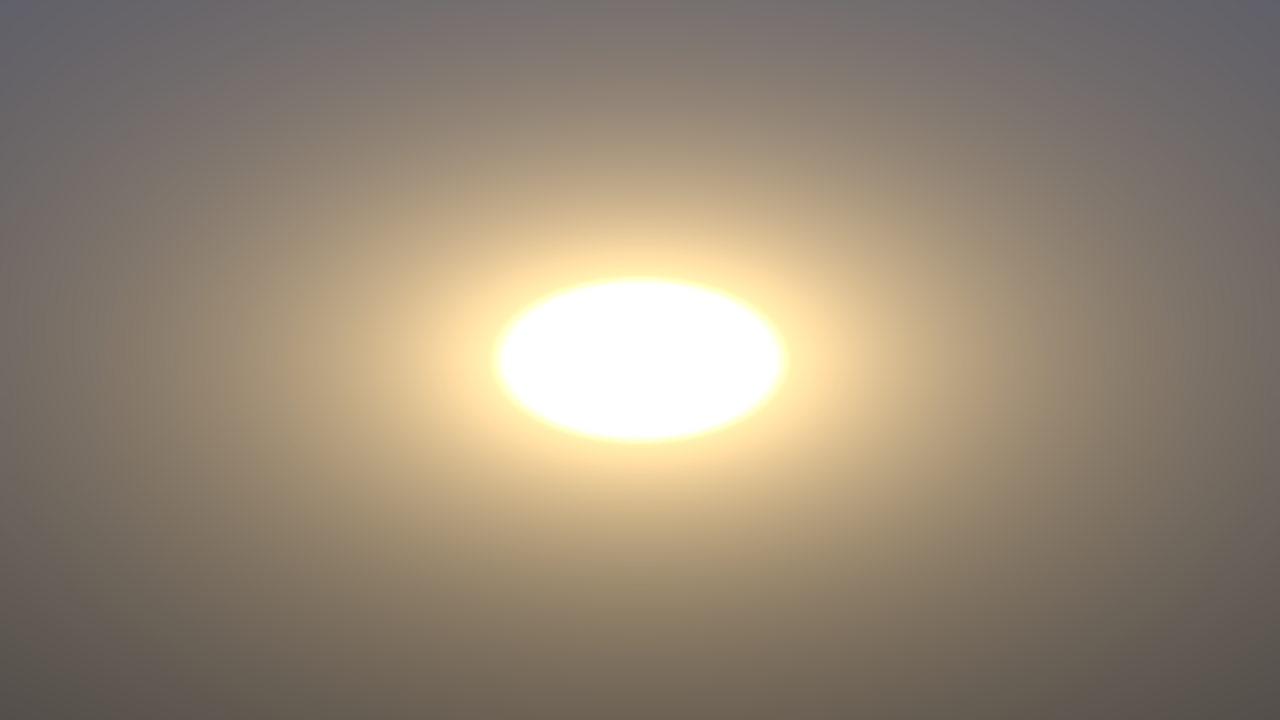
\includegraphics[width=0.82\textwidth]{captura_execucao.png}
    \caption{Captura de tela obtida diretamente do \textit{framebuffer} durante a execução do programa em Vulkan. Demonstra a operação integrada da janela GLFW, \textit{swapchain}, alocação de comandos na GPU e execução dos \textit{shaders} SPIR-V via pipeline gráfico.}
    \label{fig:captura_execucao}
\end{figure}

\subsection{Funcionalidades Concluídas e Próximos Passos}

\textbf{Funcionalidades Implementadas e Validadas nesta Etapa:}
\begin{itemize}
    \setlength{\itemsep}{0pt}
    \item Inicialização completa da instância Vulkan e integração das camadas de validação;
    \item Seleção automática de GPU discreta de alto desempenho e criação do dispositivo lógico;
    \item Identificação e separação das filas gráficas e de apresentação;
    \item Configuração dinâmica e segura da \textit{swapchain} e instanciação das \textit{Image Views};
    \item Criação de \textit{Render Pass}, \textit{Pipeline Layout}, \textit{Framebuffers} e \textit{Pipeline Gráfico};
    \item Alocação de \textit{Command Pool} e múltiplos \textit{Command Buffers};
    \item Sincronização explícita via semáforos de aquisição/renderização e \textit{fences} de CPU-GPU;
    \item Laço principal de aquisição, gravação de comandos, submissão gráfica e apresentação na tela;
    \item Compilação e carga em memória de todos os oito \textit{shaders} SPIR-V projetados;
    \item Desalocação rigorosa e ordenada de todos os recursos da GPU no encerramento da aplicação.
\end{itemize}

\textbf{Funcionalidades para as Próximas Entregas (Técnica de Bloom Completa):}
Nas próximas etapas, o pipeline base construído aqui será expandido para materializar o fluxo completo de onze passes projetado na Entrega 2:
\begin{enumerate}
    \setlength{\itemsep}{0pt}
    \item Alocação dos anexos intermediários fora de tela (\textit{offscreen}) em ponto flutuante de 16 bits (\texttt{VK\_FORMAT\_R16G16B16A16\_SFLOAT}) para a imagem \texttt{sceneHDR};
    \item Criação da textura piramidal de \textit{Bloom} (\texttt{bloomMip[0]} a \texttt{bloomMip[4]});
    \item Configuração dos \textit{Descriptor Sets} e \textit{Uniform Buffers} (\texttt{BloomParams} e \texttt{CameraUBO});
    \item Encadeamento dos passes de \textit{downsample} e \textit{upsample} com mistura aditiva (\textit{additive blending});
    \item Inserção das barreiras de memória explícitas (\texttt{VkImageMemoryBarrier}) entre as etapas de escrita e leitura de texturas.
\end{enumerate}
\fussy

% ===============================================================

\section{Integração do Código e Boilerplate Vulkan}
\label{sec:boilerplate}
\sloppy

Esta seção documenta a quarta entrega do trabalho, cujo objetivo é a construção da infraestrutura básica (\textit{boilerplate}) da aplicação gráfica em C++20 utilizando a API Vulkan, além da integração e validação dos \textit{shaders} desenvolvidos na Entrega 3 (Seção~\ref{sec:pseudocodigo}).

A aplicação desenvolvida abre uma janela interativa, inicializa as estruturas fundamentais do Vulkan, seleciona a GPU do sistema, configura a \textit{swapchain}, aloca os \textit{command buffers}, gerencia primitivas explícitas de sincronização (semáforos e \textit{fences}) e executa o ciclo de renderização na tela. Além disso, todos os oito \textit{shaders} em SPIR-V são carregados em módulos Vulkan (\texttt{VkShaderModule}) e utilizados pelo pipeline gráfico.

\subsection{Organização Modular do Projeto}
Em conformidade com os princípios da responsabilidade única (SOLID) e do código limpo (\textit{clean code}), o projeto foi estruturado em módulos independentes na pasta \texttt{src/}:

\begin{itemize}
    \setlength{\itemsep}{0pt}
    \item \textbf{\texttt{Janela} (\texttt{Janela.hpp/cpp}):} Encapsula a biblioteca GLFW, gerenciando a criação da janela sem contexto OpenGL, redimensionamentos e a criação da superfície \texttt{VkSurfaceKHR}.
    \item \textbf{\texttt{InstanciaVulkan} (\texttt{DispositivoVulkan.hpp/cpp}):} Configura a instância global da API (\texttt{VkInstance}), consulta extensões necessárias e ativa as camadas de validação (\texttt{VK\_LAYER\_KHRONOS\_validation}) com mensagens de depuração (\texttt{VkDebugUtilsMessengerEXT}).
    \item \textbf{\texttt{DispositivoVulkan} (\texttt{DispositivoVulkan.hpp/cpp}):} Identifica as GPUs físicas disponíveis, selecionando preferencialmente dispositivos dedicados (\textit{Discrete GPU}), consulta as famílias de filas com suporte a comandos gráficos e de apresentação, e cria o dispositivo lógico (\texttt{VkDevice}).
    \item \textbf{\texttt{GerenciadorSwapchain} (\texttt{GerenciadorSwapchain.hpp/cpp}):} Negocia com a superfície o melhor formato de cores (preferencialmente \texttt{VK\_FORMAT\_B8G8R8A8\_SRGB}), o modo de apresentação (\textit{Mailbox} para \textit{triple buffering} ou \textit{FIFO}) e a resolução real dos \textit{framebuffers}, instanciando as respectivas \texttt{VkImageView}s. Trata também a recriação automática da cadeia de troca quando a janela é redimensionada.
    \item \textbf{\texttt{CarregadorShader} (\texttt{CarregadorShader.hpp/cpp}):} Lê os arquivos binários compilados em SPIR-V (\texttt{.spv}) do disco e instancia os respectivos módulos Vulkan (\texttt{VkShaderModule}), gerenciando sua validação e destruição controlada.
    \item \textbf{\texttt{PipelineGrafico} (\texttt{PipelineGrafico.hpp/cpp}):} Define o \textit{Render Pass} com transições de layout, cria os \textit{Framebuffers} vinculados às imagens da \textit{swapchain} e monta o pipeline gráfico de rasterização com estágios programáveis e estados dinâmicos (\textit{viewport} e \textit{scissor}).
    \item \textbf{\texttt{AplicacaoVulkan} (\texttt{AplicacaoVulkan.hpp/cpp}):} Orquestra o ciclo de vida completo: cria o \textit{Command Pool}, aloca os \textit{Command Buffers}, inicializa semáforos e cercas (\textit{fences}) para sincronização de múltiplos quadros em voo (\textit{frames in flight}), grava os comandos de desenho e controla o laço principal (\textit{main loop}).
\end{itemize}

\subsection{Compilação dos Shaders para SPIR-V}
Os \textit{shaders} desenvolvidos em sintaxe GLSL na Entrega 3 foram compilados para o formato binário padrão do Vulkan (SPIR-V) por meio do compilador oficial \texttt{glslc}, componente do Vulkan SDK.

Foi criado o script automatizado \texttt{compilar\_shaders.sh}, que percorre todos os arquivos \texttt{.vert} e \texttt{.frag} da pasta \texttt{shaders/} e gera as saídas equivalentes em \texttt{shaders/spv/}. Além disso, o sistema de build \texttt{CMakeLists.txt} integra esse alvo (\texttt{compilar\_shaders}) antes da compilação do executável principal, garantindo que qualquer alteração nos \textit{shaders} seja automaticamente refletida nos binários SPIR-V.

\begin{table}[H]
    \centering
    \caption{\textit{Shaders} SPIR-V integrados e carregados na aplicação Vulkan.}
    \label{tab:shaders_spv}
    \vspace{4pt}
    \small
    \begin{tabular}{l l l p{6.5cm}}
        \toprule
        \textbf{Arquivo Fonte} & \textbf{Binário SPIR-V} & \textbf{Estágio} & \textbf{Papel na Técnica de Bloom} \\
        \midrule
        \texttt{scene.vert} & \texttt{scene.vert.spv} & \textit{Vertex} & Transformação de geometria 3D da cena \\
        \texttt{scene.frag} & \texttt{scene.frag.spv} & \textit{Fragment} & Iluminação direta e saída HDR sem corte \\
        \texttt{fullscreen.vert} & \texttt{fullscreen.vert.spv} & \textit{Vertex} & Geração procedural do triângulo de tela cheia \\
        \texttt{bright.frag} & \texttt{bright.frag.spv} & \textit{Fragment} & Isolamento de altas luzes (\textit{bright pass}) \\
        \texttt{downsample.frag} & \texttt{downsample.frag.spv} & \textit{Fragment} & Redução piramidal e filtro de 13 amostras \\
        \texttt{upsample.frag} & \texttt{upsample.frag.spv} & \textit{Fragment} & Expansão piramidal e filtro tenda $3\times3$ \\
        \texttt{composite.frag} & \texttt{composite.frag.spv} & \textit{Fragment} & Composição da cena com \textit{Bloom} e \textit{Tone Mapping} \\
        \texttt{teste.frag} & \texttt{teste.frag.spv} & \textit{Fragment} & Fragmento de teste visual com gradiente e núcleo luminoso \\
        \bottomrule
    \end{tabular}
\end{table}

\subsection{Ferramentas, Bibliotecas e Ambiente de Execução}
A infraestrutura foi construída e validada no seguinte ambiente técnico:
\begin{itemize}
    \setlength{\itemsep}{0pt}
    \item \textbf{Linguagem e Padrão:} C++20 (ISO/IEC 14882:2020), utilizando recursos como \texttt{std::optional}, ponteiros inteligentes (\texttt{std::unique\_ptr}) e verificação rigorosa de tipos.
    \item \textbf{Compilador:} GNU Compiler Collection (\texttt{g++} 16.2.1 / \texttt{gcc}) com suporte a flags de otimização e checagem estrita de avisos (\texttt{-Wall -Wextra -Wpedantic}).
    \item \textbf{Sistema de Build:} CMake versão 3.20 ou superior.
    \item \textbf{Vulkan SDK / Header:} Vulkan API versão 1.3 / 1.4 (especificação 1.4.364), biblioteca carregadora \texttt{libvulkan.so.1}.
    \item \textbf{Compilador de Shaders:} \texttt{glslc} (Vulkan Shader Compiler via Google Shaderc).
    \item \textbf{Bibliotecas Auxiliares:} GLFW 3.3 (gerenciamento de janelas e contexto de superfície do sistema operacional) e GLM (álgebra linear e estruturas matriciais/vetoriais).
    \item \textbf{GPU de Execução:} NVIDIA GeForce RTX 3080 (driver proprietário versão 615.71, suporte nativo à API Vulkan 1.4).
\end{itemize}

\subsection{Instruções de Compilação e Execução}

Para compilar e executar o projeto no Linux a partir do terminal:

\begin{enumerate}
    \item \textbf{Compilação dos Shaders (opcional, já acoplada ao CMake):}
    \begin{verbatim}
    ./compilar_shaders.sh
    \end{verbatim}
    \item \textbf{Geração dos arquivos de build com CMake:}
    \begin{verbatim}
    cmake -B build
    \end{verbatim}
    \item \textbf{Compilação do executável:}
    \begin{verbatim}
    cmake --build build
    \end{verbatim}
    \item \textbf{Execução da aplicação:}
    \begin{verbatim}
    ./build/BloomVulkan
    \end{verbatim}
    Para testes automatizados sem intervenção de usuário, a aplicação aceita o parâmetro \texttt{--quadros N} (ou \texttt{--teste}), que renderiza $N$ quadros, exporta a comprovação visual e finaliza de forma limpa.
\end{enumerate}

\subsection{Comprovação Visual e Funcionamento}
Ao executar a aplicação, o Vulkan inicializa a superfície de apresentação na janela criada via GLFW e associa o pipeline gráfico aos módulos SPIR-V \texttt{fullscreen.vert.spv} e \texttt{teste.frag.spv}. 

O \texttt{fullscreen.vert} gera dinamicamente as coordenadas do triângulo de tela cheia sem necessidade de \textit{vertex buffer} físico, e o \textit{fragment shader} interpola as coordenadas UV de tela cheia, desenhando um gradiente de luminância e um núcleo emissivo incandescente central. A Figura~\ref{fig:captura_execucao} ilustra a captura de tela direta gerada na renderização da GPU.

\begin{figure}[H]
    \centering
    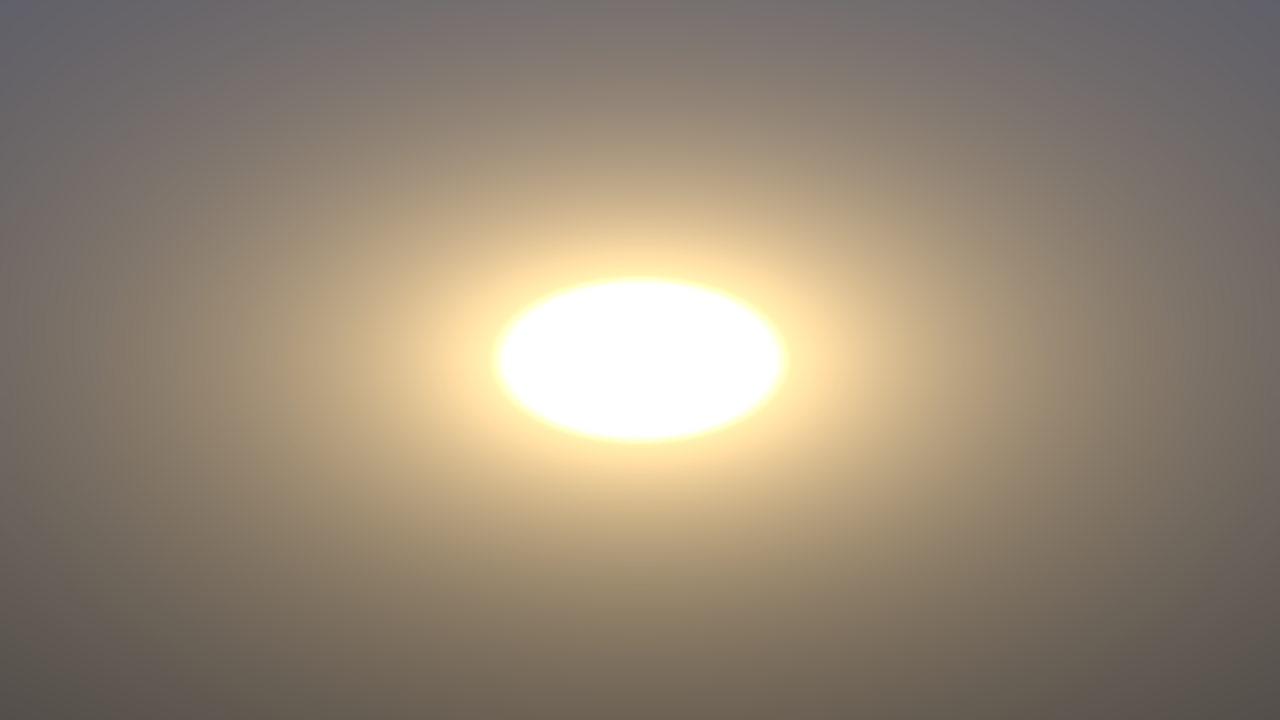
\includegraphics[width=0.82\textwidth]{captura_execucao.png}
    \caption{Captura de tela obtida diretamente do \textit{framebuffer} durante a execução do programa em Vulkan. Demonstra a operação integrada da janela GLFW, \textit{swapchain}, alocação de comandos na GPU e execução dos \textit{shaders} SPIR-V via pipeline gráfico.}
    \label{fig:captura_execucao}
\end{figure}

\subsection{Funcionalidades Concluídas e Próximos Passos}

\textbf{Funcionalidades Implementadas e Validadas nesta Etapa:}
\begin{itemize}
    \setlength{\itemsep}{0pt}
    \item Inicialização completa da instância Vulkan e integração das camadas de validação;
    \item Seleção automática de GPU discreta de alto desempenho e criação do dispositivo lógico;
    \item Identificação e separação das filas gráficas e de apresentação;
    \item Configuração dinâmica e segura da \textit{swapchain} e instanciação das \textit{Image Views};
    \item Criação de \textit{Render Pass}, \textit{Pipeline Layout}, \textit{Framebuffers} e \textit{Pipeline Gráfico};
    \item Alocação de \textit{Command Pool} e múltiplos \textit{Command Buffers};
    \item Sincronização explícita via semáforos de aquisição/renderização e \textit{fences} de CPU-GPU;
    \item Laço principal de aquisição, gravação de comandos, submissão gráfica e apresentação na tela;
    \item Compilação e carga em memória de todos os oito \textit{shaders} SPIR-V projetados;
    \item Desalocação rigorosa e ordenada de todos os recursos da GPU no encerramento da aplicação.
\end{itemize}

\textbf{Funcionalidades para as Próximas Entregas (Técnica de Bloom Completa):}
Nas próximas etapas, o pipeline base construído aqui será expandido para materializar o fluxo completo de onze passes projetado na Entrega 2:
\begin{enumerate}
    \setlength{\itemsep}{0pt}
    \item Alocação dos anexos intermediários fora de tela (\textit{offscreen}) em ponto flutuante de 16 bits (\texttt{VK\_FORMAT\_R16G16B16A16\_SFLOAT}) para a imagem \texttt{sceneHDR};
    \item Criação da textura piramidal de \textit{Bloom} (\texttt{bloomMip[0]} a \texttt{bloomMip[4]});
    \item Configuração dos \textit{Descriptor Sets} e \textit{Uniform Buffers} (\texttt{BloomParams} e \texttt{CameraUBO});
    \item Encadeamento dos passes de \textit{downsample} e \textit{upsample} com mistura aditiva (\textit{additive blending});
    \item Inserção das barreiras de memória explícitas (\texttt{VkImageMemoryBarrier}) entre as etapas de escrita e leitura de texturas.
\end{enumerate}
\fussy

% ===============================================================

\section{Integração do Código e Boilerplate Vulkan}
\label{sec:boilerplate}
\sloppy

Esta seção documenta a quarta entrega do trabalho, cujo objetivo é a construção da infraestrutura básica (\textit{boilerplate}) da aplicação gráfica em C++20 utilizando a API Vulkan, além da integração e validação dos \textit{shaders} desenvolvidos na Entrega 3 (Seção~\ref{sec:pseudocodigo}).

A aplicação desenvolvida abre uma janela interativa, inicializa as estruturas fundamentais do Vulkan, seleciona a GPU do sistema, configura a \textit{swapchain}, aloca os \textit{command buffers}, gerencia primitivas explícitas de sincronização (semáforos e \textit{fences}) e executa o ciclo de renderização na tela. Além disso, todos os oito \textit{shaders} em SPIR-V são carregados em módulos Vulkan (\texttt{VkShaderModule}) e utilizados pelo pipeline gráfico.

\subsection{Organização Modular do Projeto}
Em conformidade com os princípios da responsabilidade única (SOLID) e do código limpo (\textit{clean code}), o projeto foi estruturado em módulos independentes na pasta \texttt{src/}:

\begin{itemize}
    \setlength{\itemsep}{0pt}
    \item \textbf{\texttt{Janela} (\texttt{Janela.hpp/cpp}):} Encapsula a biblioteca GLFW, gerenciando a criação da janela sem contexto OpenGL, redimensionamentos e a criação da superfície \texttt{VkSurfaceKHR}.
    \item \textbf{\texttt{InstanciaVulkan} (\texttt{DispositivoVulkan.hpp/cpp}):} Configura a instância global da API (\texttt{VkInstance}), consulta extensões necessárias e ativa as camadas de validação (\texttt{VK\_LAYER\_KHRONOS\_validation}) com mensagens de depuração (\texttt{VkDebugUtilsMessengerEXT}).
    \item \textbf{\texttt{DispositivoVulkan} (\texttt{DispositivoVulkan.hpp/cpp}):} Identifica as GPUs físicas disponíveis, selecionando preferencialmente dispositivos dedicados (\textit{Discrete GPU}), consulta as famílias de filas com suporte a comandos gráficos e de apresentação, e cria o dispositivo lógico (\texttt{VkDevice}).
    \item \textbf{\texttt{GerenciadorSwapchain} (\texttt{GerenciadorSwapchain.hpp/cpp}):} Negocia com a superfície o melhor formato de cores (preferencialmente \texttt{VK\_FORMAT\_B8G8R8A8\_SRGB}), o modo de apresentação (\textit{Mailbox} para \textit{triple buffering} ou \textit{FIFO}) e a resolução real dos \textit{framebuffers}, instanciando as respectivas \texttt{VkImageView}s. Trata também a recriação automática da cadeia de troca quando a janela é redimensionada.
    \item \textbf{\texttt{CarregadorShader} (\texttt{CarregadorShader.hpp/cpp}):} Lê os arquivos binários compilados em SPIR-V (\texttt{.spv}) do disco e instancia os respectivos módulos Vulkan (\texttt{VkShaderModule}), gerenciando sua validação e destruição controlada.
    \item \textbf{\texttt{PipelineGrafico} (\texttt{PipelineGrafico.hpp/cpp}):} Define o \textit{Render Pass} com transições de layout, cria os \textit{Framebuffers} vinculados às imagens da \textit{swapchain} e monta o pipeline gráfico de rasterização com estágios programáveis e estados dinâmicos (\textit{viewport} e \textit{scissor}).
    \item \textbf{\texttt{AplicacaoVulkan} (\texttt{AplicacaoVulkan.hpp/cpp}):} Orquestra o ciclo de vida completo: cria o \textit{Command Pool}, aloca os \textit{Command Buffers}, inicializa semáforos e cercas (\textit{fences}) para sincronização de múltiplos quadros em voo (\textit{frames in flight}), grava os comandos de desenho e controla o laço principal (\textit{main loop}).
\end{itemize}

\subsection{Compilação dos Shaders para SPIR-V}
Os \textit{shaders} desenvolvidos em sintaxe GLSL na Entrega 3 foram compilados para o formato binário padrão do Vulkan (SPIR-V) por meio do compilador oficial \texttt{glslc}, componente do Vulkan SDK.

Foi criado o script automatizado \texttt{compilar\_shaders.sh}, que percorre todos os arquivos \texttt{.vert} e \texttt{.frag} da pasta \texttt{shaders/} e gera as saídas equivalentes em \texttt{shaders/spv/}. Além disso, o sistema de build \texttt{CMakeLists.txt} integra esse alvo (\texttt{compilar\_shaders}) antes da compilação do executável principal, garantindo que qualquer alteração nos \textit{shaders} seja automaticamente refletida nos binários SPIR-V.

\begin{table}[H]
    \centering
    \caption{\textit{Shaders} SPIR-V integrados e carregados na aplicação Vulkan.}
    \label{tab:shaders_spv}
    \vspace{4pt}
    \small
    \begin{tabular}{l l l p{6.5cm}}
        \toprule
        \textbf{Arquivo Fonte} & \textbf{Binário SPIR-V} & \textbf{Estágio} & \textbf{Papel na Técnica de Bloom} \\
        \midrule
        \texttt{scene.vert} & \texttt{scene.vert.spv} & \textit{Vertex} & Transformação de geometria 3D da cena \\
        \texttt{scene.frag} & \texttt{scene.frag.spv} & \textit{Fragment} & Iluminação direta e saída HDR sem corte \\
        \texttt{fullscreen.vert} & \texttt{fullscreen.vert.spv} & \textit{Vertex} & Geração procedural do triângulo de tela cheia \\
        \texttt{bright.frag} & \texttt{bright.frag.spv} & \textit{Fragment} & Isolamento de altas luzes (\textit{bright pass}) \\
        \texttt{downsample.frag} & \texttt{downsample.frag.spv} & \textit{Fragment} & Redução piramidal e filtro de 13 amostras \\
        \texttt{upsample.frag} & \texttt{upsample.frag.spv} & \textit{Fragment} & Expansão piramidal e filtro tenda $3\times3$ \\
        \texttt{composite.frag} & \texttt{composite.frag.spv} & \textit{Fragment} & Composição da cena com \textit{Bloom} e \textit{Tone Mapping} \\
        \texttt{teste.frag} & \texttt{teste.frag.spv} & \textit{Fragment} & Fragmento de teste visual com gradiente e núcleo luminoso \\
        \bottomrule
    \end{tabular}
\end{table}

\subsection{Ferramentas, Bibliotecas e Ambiente de Execução}
A infraestrutura foi construída e validada no seguinte ambiente técnico:
\begin{itemize}
    \setlength{\itemsep}{0pt}
    \item \textbf{Linguagem e Padrão:} C++20 (ISO/IEC 14882:2020), utilizando recursos como \texttt{std::optional}, ponteiros inteligentes (\texttt{std::unique\_ptr}) e verificação rigorosa de tipos.
    \item \textbf{Compilador:} GNU Compiler Collection (\texttt{g++} 16.2.1 / \texttt{gcc}) com suporte a flags de otimização e checagem estrita de avisos (\texttt{-Wall -Wextra -Wpedantic}).
    \item \textbf{Sistema de Build:} CMake versão 3.20 ou superior.
    \item \textbf{Vulkan SDK / Header:} Vulkan API versão 1.3 / 1.4 (especificação 1.4.364), biblioteca carregadora \texttt{libvulkan.so.1}.
    \item \textbf{Compilador de Shaders:} \texttt{glslc} (Vulkan Shader Compiler via Google Shaderc).
    \item \textbf{Bibliotecas Auxiliares:} GLFW 3.3 (gerenciamento de janelas e contexto de superfície do sistema operacional) e GLM (álgebra linear e estruturas matriciais/vetoriais).
    \item \textbf{GPU de Execução:} NVIDIA GeForce RTX 3080 (driver proprietário versão 615.71, suporte nativo à API Vulkan 1.4).
\end{itemize}

\subsection{Instruções de Compilação e Execução}

Para compilar e executar o projeto no Linux a partir do terminal:

\begin{enumerate}
    \item \textbf{Compilação dos Shaders (opcional, já acoplada ao CMake):}
    \begin{verbatim}
    ./compilar_shaders.sh
    \end{verbatim}
    \item \textbf{Geração dos arquivos de build com CMake:}
    \begin{verbatim}
    cmake -B build
    \end{verbatim}
    \item \textbf{Compilação do executável:}
    \begin{verbatim}
    cmake --build build
    \end{verbatim}
    \item \textbf{Execução da aplicação:}
    \begin{verbatim}
    ./build/BloomVulkan
    \end{verbatim}
    Para testes automatizados sem intervenção de usuário, a aplicação aceita o parâmetro \texttt{--quadros N} (ou \texttt{--teste}), que renderiza $N$ quadros, exporta a comprovação visual e finaliza de forma limpa.
\end{enumerate}

\subsection{Comprovação Visual e Funcionamento}
Ao executar a aplicação, o Vulkan inicializa a superfície de apresentação na janela criada via GLFW e associa o pipeline gráfico aos módulos SPIR-V \texttt{fullscreen.vert.spv} e \texttt{teste.frag.spv}. 

O \texttt{fullscreen.vert} gera dinamicamente as coordenadas do triângulo de tela cheia sem necessidade de \textit{vertex buffer} físico, e o \textit{fragment shader} interpola as coordenadas UV de tela cheia, desenhando um gradiente de luminância e um núcleo emissivo incandescente central. A Figura~\ref{fig:captura_execucao} ilustra a captura de tela direta gerada na renderização da GPU.

\begin{figure}[H]
    \centering
    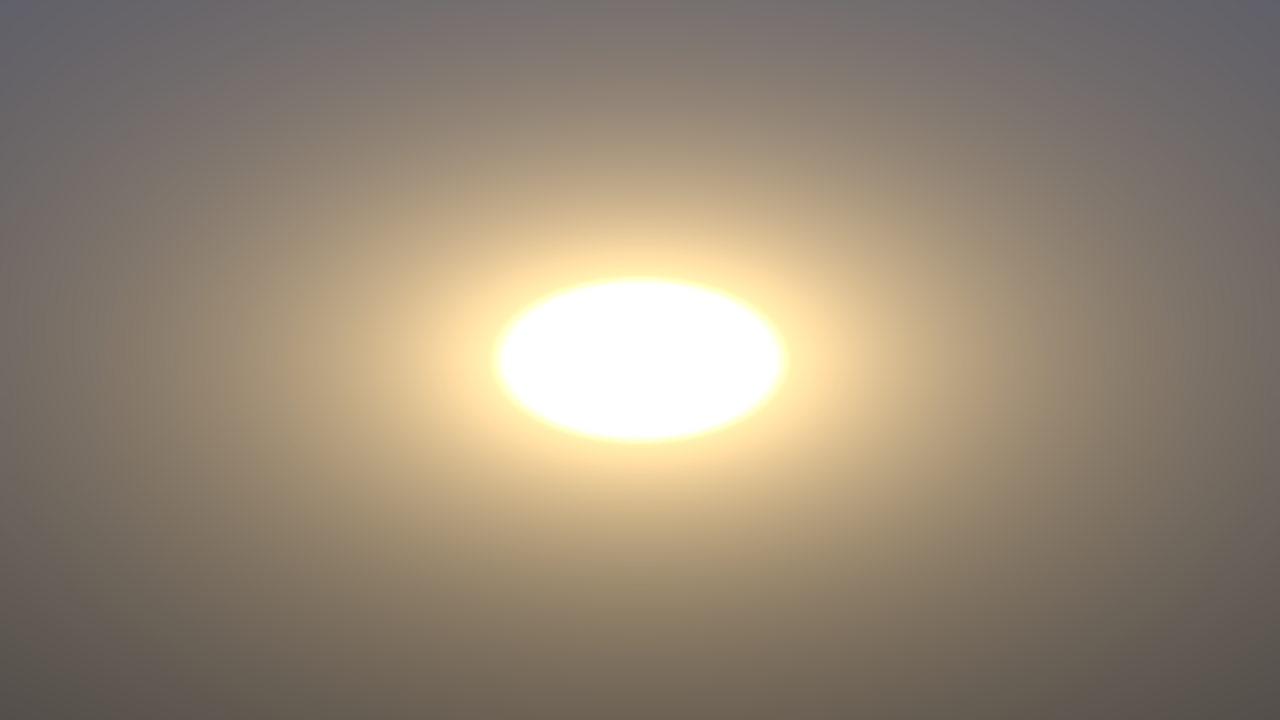
\includegraphics[width=0.82\textwidth]{captura_execucao.png}
    \caption{Captura de tela obtida diretamente do \textit{framebuffer} durante a execução do programa em Vulkan. Demonstra a operação integrada da janela GLFW, \textit{swapchain}, alocação de comandos na GPU e execução dos \textit{shaders} SPIR-V via pipeline gráfico.}
    \label{fig:captura_execucao}
\end{figure}

\subsection{Funcionalidades Concluídas e Próximos Passos}

\textbf{Funcionalidades Implementadas e Validadas nesta Etapa:}
\begin{itemize}
    \setlength{\itemsep}{0pt}
    \item Inicialização completa da instância Vulkan e integração das camadas de validação;
    \item Seleção automática de GPU discreta de alto desempenho e criação do dispositivo lógico;
    \item Identificação e separação das filas gráficas e de apresentação;
    \item Configuração dinâmica e segura da \textit{swapchain} e instanciação das \textit{Image Views};
    \item Criação de \textit{Render Pass}, \textit{Pipeline Layout}, \textit{Framebuffers} e \textit{Pipeline Gráfico};
    \item Alocação de \textit{Command Pool} e múltiplos \textit{Command Buffers};
    \item Sincronização explícita via semáforos de aquisição/renderização e \textit{fences} de CPU-GPU;
    \item Laço principal de aquisição, gravação de comandos, submissão gráfica e apresentação na tela;
    \item Compilação e carga em memória de todos os oito \textit{shaders} SPIR-V projetados;
    \item Desalocação rigorosa e ordenada de todos os recursos da GPU no encerramento da aplicação.
\end{itemize}

\textbf{Funcionalidades para as Próximas Entregas (Técnica de Bloom Completa):}
Nas próximas etapas, o pipeline base construído aqui será expandido para materializar o fluxo completo de onze passes projetado na Entrega 2:
\begin{enumerate}
    \setlength{\itemsep}{0pt}
    \item Alocação dos anexos intermediários fora de tela (\textit{offscreen}) em ponto flutuante de 16 bits (\texttt{VK\_FORMAT\_R16G16B16A16\_SFLOAT}) para a imagem \texttt{sceneHDR};
    \item Criação da textura piramidal de \textit{Bloom} (\texttt{bloomMip[0]} a \texttt{bloomMip[4]});
    \item Configuração dos \textit{Descriptor Sets} e \textit{Uniform Buffers} (\texttt{BloomParams} e \texttt{CameraUBO});
    \item Encadeamento dos passes de \textit{downsample} e \textit{upsample} com mistura aditiva (\textit{additive blending});
    \item Inserção das barreiras de memória explícitas (\texttt{VkImageMemoryBarrier}) entre as etapas de escrita e leitura de texturas.
\end{enumerate}
\fussy


% Entrega 5: protótipo funcional completo do Bloom
% ===============================================================
% Entrega 5: Prototipo Funcional Completo do Bloom em Vulkan
% Incluido no main.tex com % ===============================================================
% Entrega 5: Prototipo Funcional Completo do Bloom em Vulkan
% Incluido no main.tex com % ===============================================================
% Entrega 5: Prototipo Funcional Completo do Bloom em Vulkan
% Incluido no main.tex com \input{entrega5}
% ===============================================================

\section{Protótipo Funcional Completo em Vulkan}
\label{sec:prototipo}
\sloppy

Esta seção documenta a entrega do protótipo funcional completo da técnica de \textit{Bloom} e pós-processamento em tempo real. O código desenvolvido integra a arquitetura de 11 passes e 5 \textit{render passes} projetada na Entrega 2 (Seção~\ref{sec:arquitetura}) aos \textit{shaders} em GLSL compilados para SPIR-V da Entrega 3 (Seção~\ref{sec:pseudocodigo}), executando sobre o \textit{boilerplate} construído na Entrega 4 (Seção~\ref{sec:boilerplate}).

\subsection{Arquitetura e Fluxo de Execução na GPU}
O protótipo executa o ciclo completo de pós-processamento gráfico em tempo real para cada quadro apresentado:

\begin{enumerate}
    \setlength{\itemsep}{0pt}
    \item \textbf{Passe 0 (Cena 3D HDR):} Renderiza um modelo tridimensional rotativo com iluminação difusa Lambertiana e áreas de emissão de alta intensidade (\textit{neon}). A saída é gravada em ponto flutuante de 16 bits na imagem \texttt{sceneHDR} (\texttt{VK\_FORMAT\_R16G16B16A16\_SFLOAT}) com suporte a teste de profundidade via \texttt{depthImage}.
    \item \textbf{Barreira B1:} Transiciona a imagem \texttt{sceneHDR} do layout \texttt{COLOR\_ATTACHMENT\_OPTIMAL} para \texttt{SHADER\_READ\_ONLY\_OPTIMAL}.
    \item \textbf{Passe 1 (Bright Pass):} Executa o \texttt{bright.frag} sobre o triângulo de tela cheia, avaliando a luminância de cada bloco $2\times2$ e aplicando o corte suave (\textit{soft knee}, Equação~\ref{eq:softknee}) para isolar fragmentos com luminância superior a $1.0$, escrevendo em \texttt{bloomMip[0]} com metade da resolução nativa.
    \item \textbf{Barreira B2:} Transiciona \texttt{bloomMip[0]} para leitura como textura.
    \item \textbf{Passes 2 a 5 (Downsample Piramidal):} Encadeia 4 execuções do \texttt{downsample.frag} utilizando o filtro de 13 amostras (Equação~\ref{eq:gauss}), gerando progressivamente os níveis \texttt{bloomMip[1]} a \texttt{bloomMip[4]} com resoluções decrescentes e aplicando as respectivas barreiras de sincronização B3 a B6.
    \item \textbf{Passes 6 a 9 (Upsample Piramidal com Mistura Aditiva):} Encadeia 4 execuções do \texttt{upsample.frag} com o filtro tenda $3\times3$, interpolando os níveis menores e acumulando os dados nos níveis maiores via \textit{Additive Blending} (\texttt{VK\_BLEND\_FACTOR\_ONE} na origem e no destino) com as barreiras B7 a B10. Ao término do Passe 9, o nível \texttt{bloomMip[0]} armazena o halo de dispersão volumétrica completo.
    \item \textbf{Passe 10 (Composição e Tone Mapping):} Executa o \texttt{composite.frag}, combinando aditivamente a cena original \texttt{sceneHDR} com o halo de \textit{Bloom} ponderado pelo fator de intensidade $\alpha$, aplicando o mapeamento tonal de Reinhard (Equação~\ref{eq:reinhard}) e gravando o resultado final na imagem da \textit{swapchain} para apresentação ao monitor.
\end{enumerate}

\subsection{Comprovação Visual e Análise Comparativa}
Para comprovar cientificamente o funcionamento da técnica, o protótipo inclui um mecanismo de controle dinâmico que permite ligar e desligar o \textit{Bloom} em tempo real. A Figura~\ref{fig:comparativo_bloom} apresenta a comparação direta capturada da memória da GPU.

\begin{figure}[H]
    \centering
    \begin{minipage}{0.48\textwidth}
        \centering
        
\includegraphics[width=\linewidth]{captura_bloom_desativado.png}
        \textbf{(a) Sem Bloom (LDR puro)}
    \end{minipage}
    \hfill
    \begin{minipage}{0.48\textwidth}
        \centering
        
\includegraphics[width=\linewidth]{captura_bloom_ativo.png}
        \textbf{(b) Com Bloom Ativo}
    \end{minipage}
    \caption{Comparação direta gerada pelo protótipo Vulkan. Em (a), a faixa incandescente sofre corte abrupto sem simulação de dispersão; em (b), o pipeline completo de 11 passes produz o espalhamento suave da luz (\textit{light bleeding}) ao redor do objeto, conferindo a percepção física de extrema luminância.}
    \label{fig:comparativo_bloom}
\end{figure}

\subsection{Interatividade e Usabilidade do Protótipo}
O protótipo permite intervenção direta do usuário em tempo de execução através das seguintes teclas:
\begin{itemize}
    \setlength{\itemsep}{0pt}
    \item \textbf{Barra de Espaço:} Alterna instantaneamente entre o modo com \textit{Bloom} ativo e o modo desativado, viabilizando a demonstração comparativa ao vivo.
    \item \textbf{Teclas \texttt{+} e \texttt{-}:} Aumentam e diminuem a intensidade do espalhamento luminoso ($\alpha$).
    \item \textbf{Tecla \texttt{ESC}:} Encerra a aplicação de forma limpa, garantindo a destruição ordenada de todos os semáforos, \textit{fences}, imagens e \textit{buffers} alocados na GPU.
\end{itemize}
\fussy

% ===============================================================

\section{Protótipo Funcional Completo em Vulkan}
\label{sec:prototipo}
\sloppy

Esta seção documenta a entrega do protótipo funcional completo da técnica de \textit{Bloom} e pós-processamento em tempo real. O código desenvolvido integra a arquitetura de 11 passes e 5 \textit{render passes} projetada na Entrega 2 (Seção~\ref{sec:arquitetura}) aos \textit{shaders} em GLSL compilados para SPIR-V da Entrega 3 (Seção~\ref{sec:pseudocodigo}), executando sobre o \textit{boilerplate} construído na Entrega 4 (Seção~\ref{sec:boilerplate}).

\subsection{Arquitetura e Fluxo de Execução na GPU}
O protótipo executa o ciclo completo de pós-processamento gráfico em tempo real para cada quadro apresentado:

\begin{enumerate}
    \setlength{\itemsep}{0pt}
    \item \textbf{Passe 0 (Cena 3D HDR):} Renderiza um modelo tridimensional rotativo com iluminação difusa Lambertiana e áreas de emissão de alta intensidade (\textit{neon}). A saída é gravada em ponto flutuante de 16 bits na imagem \texttt{sceneHDR} (\texttt{VK\_FORMAT\_R16G16B16A16\_SFLOAT}) com suporte a teste de profundidade via \texttt{depthImage}.
    \item \textbf{Barreira B1:} Transiciona a imagem \texttt{sceneHDR} do layout \texttt{COLOR\_ATTACHMENT\_OPTIMAL} para \texttt{SHADER\_READ\_ONLY\_OPTIMAL}.
    \item \textbf{Passe 1 (Bright Pass):} Executa o \texttt{bright.frag} sobre o triângulo de tela cheia, avaliando a luminância de cada bloco $2\times2$ e aplicando o corte suave (\textit{soft knee}, Equação~\ref{eq:softknee}) para isolar fragmentos com luminância superior a $1.0$, escrevendo em \texttt{bloomMip[0]} com metade da resolução nativa.
    \item \textbf{Barreira B2:} Transiciona \texttt{bloomMip[0]} para leitura como textura.
    \item \textbf{Passes 2 a 5 (Downsample Piramidal):} Encadeia 4 execuções do \texttt{downsample.frag} utilizando o filtro de 13 amostras (Equação~\ref{eq:gauss}), gerando progressivamente os níveis \texttt{bloomMip[1]} a \texttt{bloomMip[4]} com resoluções decrescentes e aplicando as respectivas barreiras de sincronização B3 a B6.
    \item \textbf{Passes 6 a 9 (Upsample Piramidal com Mistura Aditiva):} Encadeia 4 execuções do \texttt{upsample.frag} com o filtro tenda $3\times3$, interpolando os níveis menores e acumulando os dados nos níveis maiores via \textit{Additive Blending} (\texttt{VK\_BLEND\_FACTOR\_ONE} na origem e no destino) com as barreiras B7 a B10. Ao término do Passe 9, o nível \texttt{bloomMip[0]} armazena o halo de dispersão volumétrica completo.
    \item \textbf{Passe 10 (Composição e Tone Mapping):} Executa o \texttt{composite.frag}, combinando aditivamente a cena original \texttt{sceneHDR} com o halo de \textit{Bloom} ponderado pelo fator de intensidade $\alpha$, aplicando o mapeamento tonal de Reinhard (Equação~\ref{eq:reinhard}) e gravando o resultado final na imagem da \textit{swapchain} para apresentação ao monitor.
\end{enumerate}

\subsection{Comprovação Visual e Análise Comparativa}
Para comprovar cientificamente o funcionamento da técnica, o protótipo inclui um mecanismo de controle dinâmico que permite ligar e desligar o \textit{Bloom} em tempo real. A Figura~\ref{fig:comparativo_bloom} apresenta a comparação direta capturada da memória da GPU.

\begin{figure}[H]
    \centering
    \begin{minipage}{0.48\textwidth}
        \centering
        
\includegraphics[width=\linewidth]{captura_bloom_desativado.png}
        \textbf{(a) Sem Bloom (LDR puro)}
    \end{minipage}
    \hfill
    \begin{minipage}{0.48\textwidth}
        \centering
        
\includegraphics[width=\linewidth]{captura_bloom_ativo.png}
        \textbf{(b) Com Bloom Ativo}
    \end{minipage}
    \caption{Comparação direta gerada pelo protótipo Vulkan. Em (a), a faixa incandescente sofre corte abrupto sem simulação de dispersão; em (b), o pipeline completo de 11 passes produz o espalhamento suave da luz (\textit{light bleeding}) ao redor do objeto, conferindo a percepção física de extrema luminância.}
    \label{fig:comparativo_bloom}
\end{figure}

\subsection{Interatividade e Usabilidade do Protótipo}
O protótipo permite intervenção direta do usuário em tempo de execução através das seguintes teclas:
\begin{itemize}
    \setlength{\itemsep}{0pt}
    \item \textbf{Barra de Espaço:} Alterna instantaneamente entre o modo com \textit{Bloom} ativo e o modo desativado, viabilizando a demonstração comparativa ao vivo.
    \item \textbf{Teclas \texttt{+} e \texttt{-}:} Aumentam e diminuem a intensidade do espalhamento luminoso ($\alpha$).
    \item \textbf{Tecla \texttt{ESC}:} Encerra a aplicação de forma limpa, garantindo a destruição ordenada de todos os semáforos, \textit{fences}, imagens e \textit{buffers} alocados na GPU.
\end{itemize}
\fussy

% ===============================================================

\section{Protótipo Funcional Completo em Vulkan}
\label{sec:prototipo}
\sloppy

Esta seção documenta a entrega do protótipo funcional completo da técnica de \textit{Bloom} e pós-processamento em tempo real. O código desenvolvido integra a arquitetura de 11 passes e 5 \textit{render passes} projetada na Entrega 2 (Seção~\ref{sec:arquitetura}) aos \textit{shaders} em GLSL compilados para SPIR-V da Entrega 3 (Seção~\ref{sec:pseudocodigo}), executando sobre o \textit{boilerplate} construído na Entrega 4 (Seção~\ref{sec:boilerplate}).

\subsection{Arquitetura e Fluxo de Execução na GPU}
O protótipo executa o ciclo completo de pós-processamento gráfico em tempo real para cada quadro apresentado:

\begin{enumerate}
    \setlength{\itemsep}{0pt}
    \item \textbf{Passe 0 (Cena 3D HDR):} Renderiza um modelo tridimensional rotativo com iluminação difusa Lambertiana e áreas de emissão de alta intensidade (\textit{neon}). A saída é gravada em ponto flutuante de 16 bits na imagem \texttt{sceneHDR} (\texttt{VK\_FORMAT\_R16G16B16A16\_SFLOAT}) com suporte a teste de profundidade via \texttt{depthImage}.
    \item \textbf{Barreira B1:} Transiciona a imagem \texttt{sceneHDR} do layout \texttt{COLOR\_ATTACHMENT\_OPTIMAL} para \texttt{SHADER\_READ\_ONLY\_OPTIMAL}.
    \item \textbf{Passe 1 (Bright Pass):} Executa o \texttt{bright.frag} sobre o triângulo de tela cheia, avaliando a luminância de cada bloco $2\times2$ e aplicando o corte suave (\textit{soft knee}, Equação~\ref{eq:softknee}) para isolar fragmentos com luminância superior a $1.0$, escrevendo em \texttt{bloomMip[0]} com metade da resolução nativa.
    \item \textbf{Barreira B2:} Transiciona \texttt{bloomMip[0]} para leitura como textura.
    \item \textbf{Passes 2 a 5 (Downsample Piramidal):} Encadeia 4 execuções do \texttt{downsample.frag} utilizando o filtro de 13 amostras (Equação~\ref{eq:gauss}), gerando progressivamente os níveis \texttt{bloomMip[1]} a \texttt{bloomMip[4]} com resoluções decrescentes e aplicando as respectivas barreiras de sincronização B3 a B6.
    \item \textbf{Passes 6 a 9 (Upsample Piramidal com Mistura Aditiva):} Encadeia 4 execuções do \texttt{upsample.frag} com o filtro tenda $3\times3$, interpolando os níveis menores e acumulando os dados nos níveis maiores via \textit{Additive Blending} (\texttt{VK\_BLEND\_FACTOR\_ONE} na origem e no destino) com as barreiras B7 a B10. Ao término do Passe 9, o nível \texttt{bloomMip[0]} armazena o halo de dispersão volumétrica completo.
    \item \textbf{Passe 10 (Composição e Tone Mapping):} Executa o \texttt{composite.frag}, combinando aditivamente a cena original \texttt{sceneHDR} com o halo de \textit{Bloom} ponderado pelo fator de intensidade $\alpha$, aplicando o mapeamento tonal de Reinhard (Equação~\ref{eq:reinhard}) e gravando o resultado final na imagem da \textit{swapchain} para apresentação ao monitor.
\end{enumerate}

\subsection{Comprovação Visual e Análise Comparativa}
Para comprovar cientificamente o funcionamento da técnica, o protótipo inclui um mecanismo de controle dinâmico que permite ligar e desligar o \textit{Bloom} em tempo real. A Figura~\ref{fig:comparativo_bloom} apresenta a comparação direta capturada da memória da GPU.

\begin{figure}[H]
    \centering
    \begin{minipage}{0.48\textwidth}
        \centering
        
\includegraphics[width=\linewidth]{captura_bloom_desativado.png}
        \textbf{(a) Sem Bloom (LDR puro)}
    \end{minipage}
    \hfill
    \begin{minipage}{0.48\textwidth}
        \centering
        
\includegraphics[width=\linewidth]{captura_bloom_ativo.png}
        \textbf{(b) Com Bloom Ativo}
    \end{minipage}
    \caption{Comparação direta gerada pelo protótipo Vulkan. Em (a), a faixa incandescente sofre corte abrupto sem simulação de dispersão; em (b), o pipeline completo de 11 passes produz o espalhamento suave da luz (\textit{light bleeding}) ao redor do objeto, conferindo a percepção física de extrema luminância.}
    \label{fig:comparativo_bloom}
\end{figure}

\subsection{Interatividade e Usabilidade do Protótipo}
O protótipo permite intervenção direta do usuário em tempo de execução através das seguintes teclas:
\begin{itemize}
    \setlength{\itemsep}{0pt}
    \item \textbf{Barra de Espaço:} Alterna instantaneamente entre o modo com \textit{Bloom} ativo e o modo desativado, viabilizando a demonstração comparativa ao vivo.
    \item \textbf{Teclas \texttt{+} e \texttt{-}:} Aumentam e diminuem a intensidade do espalhamento luminoso ($\alpha$).
    \item \textbf{Tecla \texttt{ESC}:} Encerra a aplicação de forma limpa, garantindo a destruição ordenada de todos os semáforos, \textit{fences}, imagens e \textit{buffers} alocados na GPU.
\end{itemize}
\fussy


\section{Conclusão}
O efeito de \textit{Bloom} consolidou-se como um pilar indispensável da renderização computacional em tempo real. Sua fundamentação em fenômenos físicos e fisiológicos de dispersão intraocular, aliada às capacidades de baixo nível da API Vulkan --- como controle explícito de barreiras de sincronização e processamento massivo via \textit{Compute Shaders} ---, viabiliza a emulação convincente de faixas dinâmicas extremas com baixo impacto de desempenho.

\begin{thebibliography}{99}

\bibitem{seetzen2004hdr}
H.~Seetzen, W.~Heidrich, W.~Stuerzlinger, G.~Ward, L.~Whitehead, M.~Trentacoste, A.~Ghosh, and A.~Vorozcovs, 
``High dynamic range display systems,'' 
\emph{ACM Transactions on Graphics (TOG)}, vol.~23, no.~3, pp. 760--768, 2004.

\bibitem{spencer1995glare}
G.~Spencer, P.~Shirley, K.~Zimmerman, and D.~P.~Greenberg, 
``Physically-based glare effects for digital images,'' 
in \emph{Proceedings of the 22nd Annual Conference on Computer Graphics and Interactive Techniques (ACM SIGGRAPH)}, pp. 325--334, 1995.

\bibitem{reinhard2002tone}
E.~Reinhard, M.~Stark, P.~Shirley, and J.~Ferwerda, 
``Photographic tone reproduction for digital images,'' 
\emph{ACM Transactions on Graphics (TOG)}, vol.~21, no.~3, pp. 267--276, 2002.

\bibitem{ignatenko2008glare}
A.~Ignatenko and A.~Barladyan, 
``Using quad-trees for acceleration of physically-based image-space rendering of glare,'' 
in \emph{Proceedings of GraphiCon'2008 (International Conference on Computer Graphics and Vision)}, pp. 128--133, 2008.

\bibitem{cadik2005naturalness}
M.~{\v{C}}ad{\'\i}k, M.~Wimmer, L.~Neumann, and P.~{\v{D}}urikoviv{\v{c}}, 
``The naturalness of reproduced high dynamic range images,'' 
in \emph{Ninth International Conference on Information Visualisation (IV'05)}, pp. 569--576, IEEE, 2005.

\end{thebibliography}

\end{document}